%%%%%%%%%%%%%%%%%%%%%%%%%%%%%%%%%%%%%%%%%%%%%%%%%%%%%%%%%%%%%%%%%%%%%%%%%%%%%%%
% Neuroimage-like layout
\documentclass[5p]{elsarticle}
\usepackage{amsmath,amsfonts,amssymb}
\usepackage{bm}
\usepackage{algorithm}
\usepackage{algorithmic}
\usepackage{url}
\usepackage[breaklinks=true,letterpaper=true,colorlinks,bookmarks=false]{hyperref}
\usepackage[table]{xcolor}

\definecolor{deep_blue}{rgb}{0,.2,.5}
\definecolor{dark_blue}{rgb}{0,.15,.5}

\hypersetup{pdftex,  % needed for pdflatex
  breaklinks=true,  % so long urls are correctly broken across lines
  colorlinks=true,
  linkcolor=dark_blue,
  citecolor=deep_blue,
}

% Float parameters, for more full pages.
\renewcommand{\topfraction}{0.9}        % max fraction of floats at top
\renewcommand{\bottomfraction}{0.8}     % max fraction of floats at bottom
\renewcommand{\textfraction}{0.07}      % allow minimal text w. figs
%   Parameters for FLOAT pages (not text pages):
\renewcommand{\floatpagefraction}{0.6}  % require fuller float pages
%    % N.B.: floatpagefraction MUST be less than topfraction !!


\def\B#1{\mathbf{#1}}
%\def\B#1{\bm{#1}}
\def\trans{^\mathsf{T}}
% A compact fraction
\def\slantfrac#1#2{\kern.1em^{#1}\kern-.1em/\kern-.1em_{#2}}

%%%%%%%%%%%%%%%%%%%%%%%%%%%%%%%%%%%%%%%%%%%%%%%%%%%%%%%%%%%%%%%%%%%%%%%%%%%%%%%%
\begin{document}

%\title{Comparing Connectomes Between Populations}
\title{Learning and comparing functional connectomes between populations}


\author[parietal,unicog,cea]{Ga\"el Varoquaux\corref{corresponding}}
\author[cmi,nki]{R. Cameron Craddock}

\cortext[corresponding]{Corresponding author}

\address[parietal]{Parietal project-team, INRIA Saclay-\^ile de France}
\address[unicog]{INSERM, U992}
\address[cea]{CEA/Neurospin b\^at 145, 91191 Gif-Sur-Yvette}
\address[cmi]{Child Mind Institute, New York, New York}
\address[nki]{Nathan Kline Institute for Psychiatric Research, Orangeburg, New York}

\begin{abstract}
    We are the champion... of the world

    Scope: rest and task-based studies. But focusing on fMRI.
\end{abstract}

\begin{keyword}
    Functional connectivity, connectome, group study, effective
    connectivity, fMRI, resting-state
\end{keyword}

\maketitle
%%%%%%%%%%%%%%%%%%%%%%%%%%%%%%%%%%%%%%%%%%%%%%%%%%%%%%%%%%%%%%%%%%%%%%%%%%%%%%%%

\sloppy % Fed up with messed-up line breaks
\section{Introduction}

Review paper giving technical guidelines.

BOLD signal during rest is typically just 5-10\% lower than during task-based
experiments (cite Raichle,  Mintun, Annu. Rev. Neurosci. 29, 449–476 (2006).)

Define what we call a functional connectome, and the term \emph{graph},
as well as its relation with an adjacency matrix.

Define a functional network

Define on-going vs evoked activity


%%%%%%%%%%%%%%%%%%%%%%%%%%%%%%%%%%%%%%%%%%%%%%%%%%%%%%%%%%%%%%%%%%%%%%%%%%%%%%%

\section{Estimating functional connectomes}

Here we discuss strategies to infer connectomes from functional brain
imaging data. We start with the choice of nodes \emph{i.e.}\ regions,
followed by signal extraction, and the estimation of graphs.

%------------------------------------------------------------------------------
\subsection{Defining regions}

The choice of regions of interests (ROIs) that defines the nodes of the
graphs can be very important both in the estimation of connectomes and
for group comparison \cite{wang2009}. Unsurprisingly, simulations have
shown that extracting signal from ROIs that did not match functional
units would lead to incorrect graph extraction \cite{smith2011}.
%
Different strategies coexist. While dense parcellations approaches cover
a large fraction of the brain \cite{achard2006, varoquaux2010c,
wang2009}, this coverage can be traded off to focus on some specific
regions, in favor of increased functional specificity and thus better
differentiation across networks \cite{greicius2003, fair2009,
varoquaux2010b, lewis2009, fransson2008, shirer2012}. In addition, while
ROIs and most often defined as a hard selection of voxels, it is also
possible to use a \emph{soft} definition, attributing weights as with
probabilistic atlases, or spatial maps of functional networks extracted
from techniques such as independent component analysis (ICA).

% XXX: discuss tradeoffs in the number of regions

\paragraph{Regions from atlases}
%
Atlases can be used to define full-brain parcellations. The most popular
choice is probably the AAL atlas \cite{tzourio-mazoyer2002a}, that
benefits from an SPM toolbox. However, it suffers from major
shortcomings; namely that \emph{i)} it was defined on a single subject
and thus does does not reflect inter-subject variability and \emph{ii)}
focuses on labeling large anatomical structures and does not match
functional layout --for instance only two regions describe the medial
part of the frontal lobe. Multi-subject probabilistic altases such as the
Harvard-Oxford atlas distributed with FSL \cite{smith2004} or the
sulci-based structural atlas used in \cite{varoquaux2010c} mitigate the
first problem, and the high number of regions defined using sulci also
somewhat circumvent the second problem (see
fig.\,\ref{fig:parcellations}).


\paragraph{Defining regions from the literature}
%
Regions can be defined from previous studies, informally or with
systematic meta-analysis. This strategy is used to define the main
resting-state networks, such as the default mode network, but may also be
useful to study connectivity in task-specific networks
\cite{grillon2012}. The common practice is to place balls of a given
radius, 5 or 10\,mm, centered at the coordinates of interest. Given that
functional networks are tightly interleaved in some parts of the cortex,
such as the parietal lobe, care must be taken not to define too many
regions that would overlap and lead to mixing of the signal.

\paragraph{FMRI-based function definition}
%
Defining regions directly from the fMRI signal brings many benefits.
First, it can capture subject-specific functional information. Second, it
also adapts to the signal at hand and it's limitations, such as
EPI-specific warps or vascular and movement artifacts that are isolated
in ICA-like approaches. The simplest approach to define task-specific
regions is to use activation maps derived from standard GLM-based
analysis in a task-driven study (see for instance \cite{poldrack2011}).
Regions are extracted by thresholding the maps, or using balls around the
activation peaks. For resting-state studies, unsupervised multivariate
analysis techniques are necessary. Clustering approaches extract
full-brain parcellations \cite{craddock2011, bellec2010, yeo2011,
thirion2006}, and have been shown to extract well-known functional
structures from rest data \cite{yeo2011}. Alternatively, decompositions
methods, such as ICA \cite{beckmann2004}, can unmixing linear
combinations of multiple effects and separate out multiple spatial maps
capturing functional networks or confounding effects. At high model
order, ICA maps define a functional parcellation \cite{kiviniemi2009}.
Extracting regions from these maps requires additional effort as they can
display fragmented spatial features and structured background noise, but
incorporating sparsity and spatial constraints in the decomposition
techniques leads to contrasted maps that outline many different
structures \cite{varoquaux2012} (see fig.\,\ref{fig:parcellations}).

%{{{------ Parcellation figure -----------------------------------------------
\begin{figure}
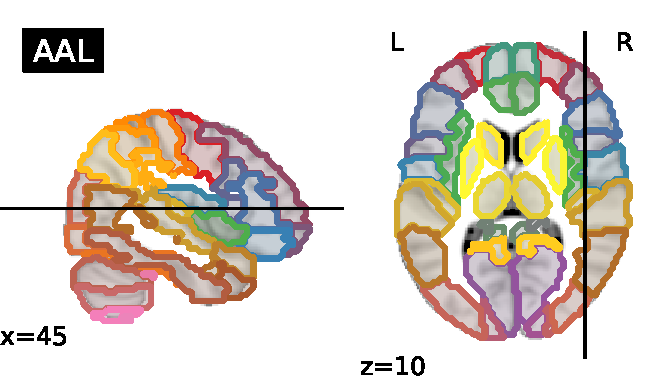
\includegraphics[width=.5\linewidth]{aal_atlas.pdf}%
\hfill%
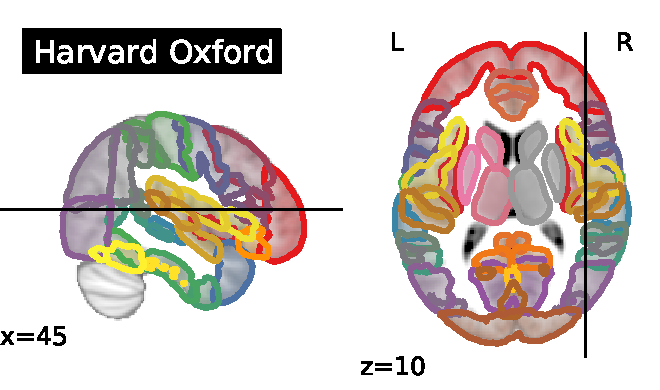
\includegraphics[width=.5\linewidth]{ho_atlas.pdf}%

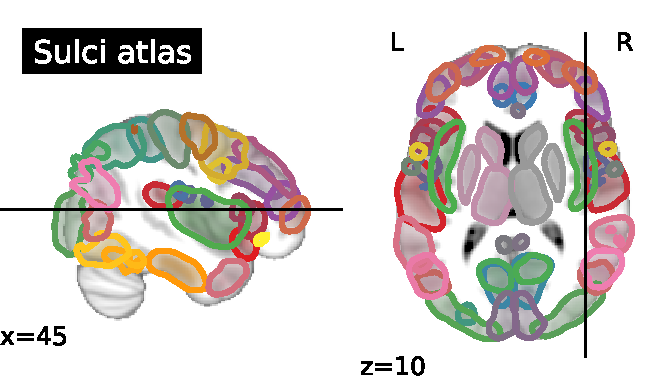
\includegraphics[width=.5\linewidth]{sulci_atlas.pdf}%
\hfill%
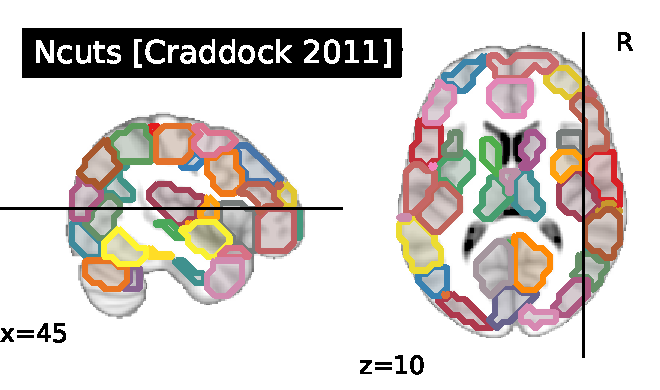
\includegraphics[width=.5\linewidth]{ncuts_atlas.pdf}%

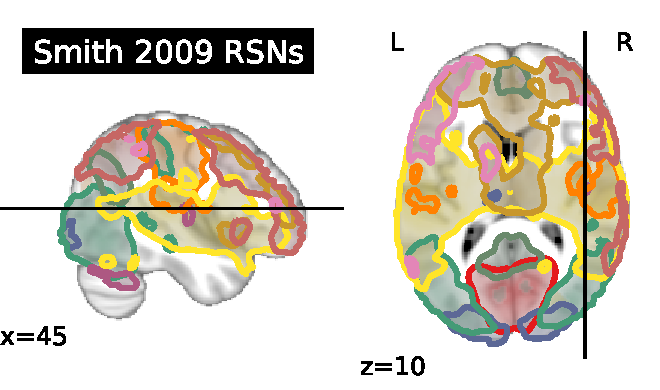
\includegraphics[width=.5\linewidth]{smith_atlas.pdf}%
\hfill%
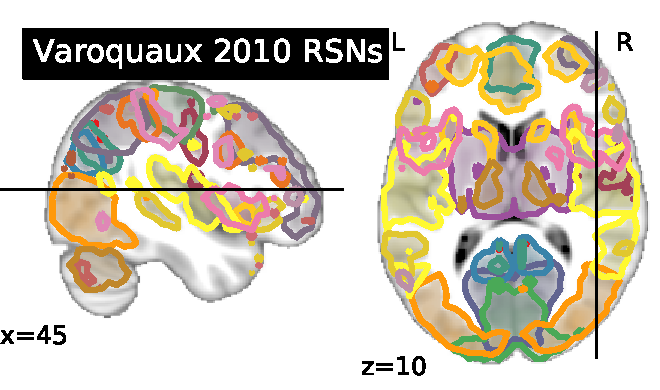
\includegraphics[width=.5\linewidth]{msdl_atlas.pdf}%

\caption{
Different full-brain parcellations: the AAL atlas
\cite{tzourio-mazoyer2002a}, the Harvard-Oxford atlas, the sucli atlas used in
\cite{varoquaux2010c}, regions extracted by Ncuts
\cite{craddock2011}, the resting-state networks extracted in
\cite{smith2009} by ICA, and in \cite{varoquaux2011} by sparse dictionary
learning.
\label{fig:parcellations}
}
\end{figure}
%---------------------------------------------------------------------------}}}

%------------------------------------------------------------------------------
\subsection{Estimating connections}

The concept of functional connectivity has be called elusive
\cite{horwitz2003}: it has many mathematical instantiations although in
essence they all strive to extract simple statistics from functional
imaging to characterize synchrony and communication between large
ensembles of neurons. Here we choose to focus on second order statistics
that can be related to Gaussian models, the simplest of which being the
correlation matrix of the signals of the different ROIs.


%{{{------ Correlation matrices figure ---------------------------------------
\begin{figure}
\newcommand{\photoframe}[1]{\setlength\fboxsep{0pt}%
{\color{black!70}\fbox{#1}\color{black}}}%
\begin{minipage}{.666\linewidth}%
    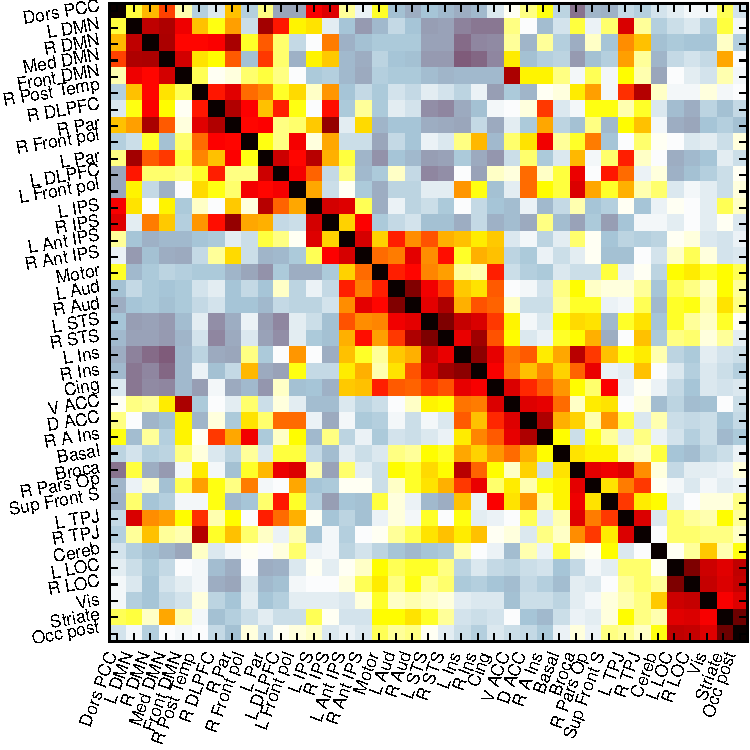
\includegraphics[width=\linewidth]{group_emp_cov.pdf}%
    \raisebox{.606\linewidth}{%
	\hspace*{-.462\linewidth}%
	\photoframe{%
	%\setlength\fboxsep{1pt}%
	\colorbox{white}{%
	\raisebox{.003\linewidth}{%
	    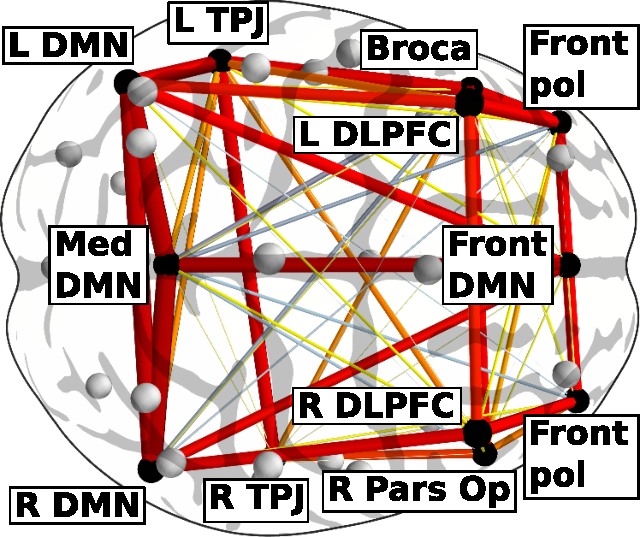
\includegraphics[width=.455\linewidth]{group_emp_cov_3d_labels}}%
	\rule{0pt}{.387\linewidth}%
	}}%
    }
\end{minipage}%
\hspace*{1pt}%
\begin{minipage}{.33\linewidth}%
    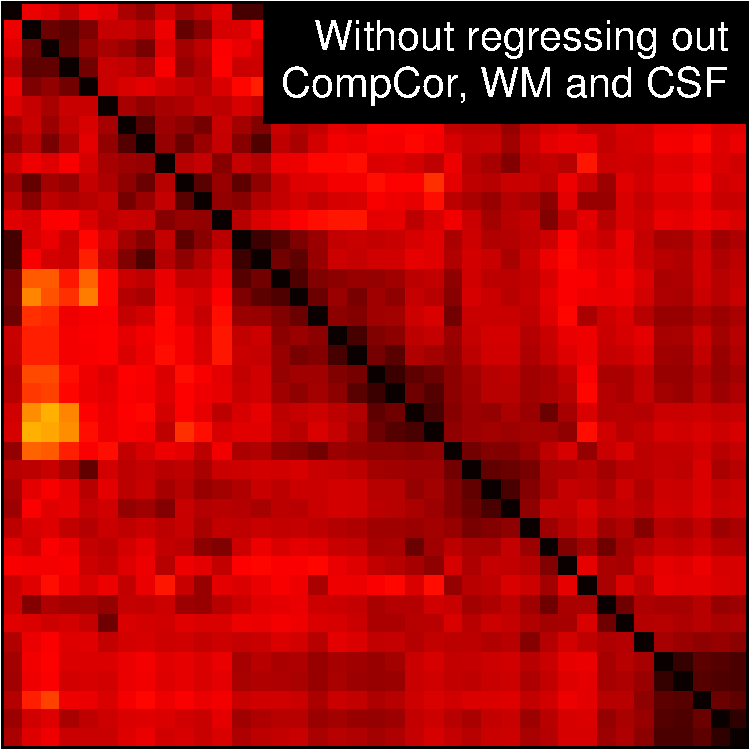
\includegraphics[width=\linewidth]{group_emp_cov_no_confounds.pdf}%

    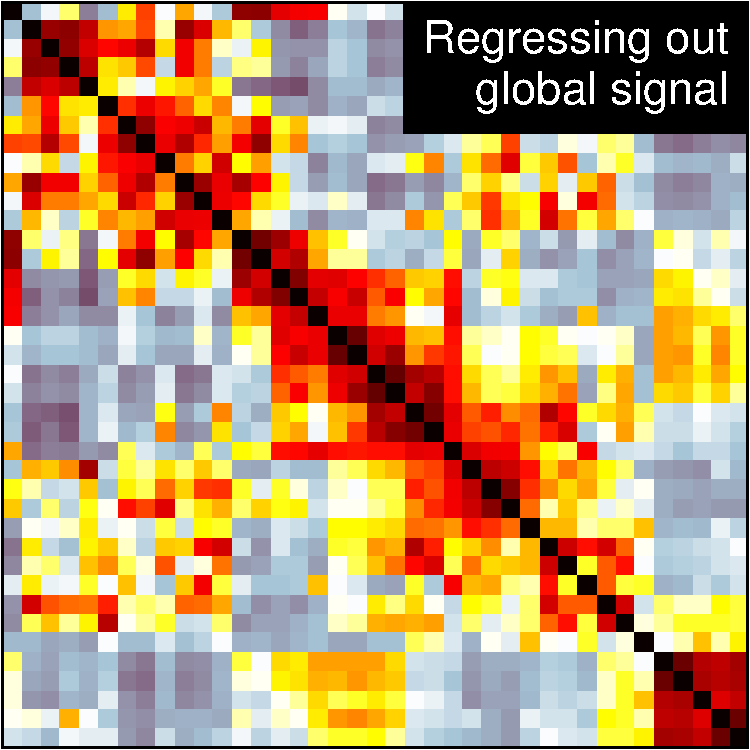
\includegraphics[width=\linewidth]{group_emp_cov_global_mean.pdf}%
\end{minipage}%

% XXX: need to give details on the dataset used here

\caption{
Correlation matrices of rest time-series extracted from the 39 main
regions of the Varoquaux 2011 \cite{varoquaux2011} parcellation with
different choices of confound regressors -- 
\textbf{Left}: regressing out CompCor signals, as well as white matter and
CSF average signals and movement parameters. The insert shows the
connections restricted to the .
-- \textbf{Upper right}: regressing out only movement parameters. -- 
\textbf{Lower right}:
regressing out movement parameters and global signal mean.
No frequency filtering was applied here.
\label{fig:correlation_matrices}
When no confounding brain signals are regressed, all regions are heavily
correlated. Regressing out common signal, in the form of well-identified
confounds or a global mean, teases out the structure.
}
\end{figure}
%---------------------------------------------------------------------------}}}

% The following paragraph is convoluted: we start to say that rest is
% from time-series, and task from beta, we go on discussing about beta
% maps, and then we move back to rest. It might need restructuring

% Horrible sentence below

\paragraph{Signal extraction}
%
Given ROIs, the next step is to extract from them a summary measure. To
study \emph{on-going} activity, \emph{e.g.}\ with rest data, signal
extraction is performed from the EPI time series; however, to study
\emph{evoked} activity with task-driven studies it can be beneficial to
run a first-level analysis, enforcing specificity of the measure
extracted to the task. With slow event-related design, task-specific
functional connectivity can be captured in trial-to-trial fluctuations in
the BOLD response, estimated using a GLM analysis with one regressor per
trial \cite{grillon2012,rissman2004}. This approach, known as beta-series
regression, has been adapted for rapid event-related designs, using
multiple GLMs to optimize deconvolution of each trial \cite{mumford2012}.
With rest datasets, it is important to regress out time series capturing
movement and other sources of structured noise, to separate on-going
activity from confounding signals. In addition to removing movement
parameters estimated during preprocessing, removing linear trends, signal
extracted from the white matter and the CSF \cite{chang2009}, as well as
using the CompCor \cite{behzadi2007} procedure gives more contrasted
correlation matrices that outline functional structures better
(fig.\,\ref{fig:correlation_matrices}). Filtering high frequencies is
often recommended, based on the initial observation that neural-related
signal are observed below 0.1\,Hz \cite{cordes2001,biswal1995}. While
high-pass and low-pass filtering decrease the impact of some confounds,
recent studies have shown that information on neural processes is present
in the full spectrum of frequencies observed
\cite{smith2012,vanoort2012}. Regressing out a good choice of confound
signals is more specific than frequency filter, and in our experience
gives more contrasted correlation matrices\footnote{Note that naive use
of filtering can induce spurious correlations \cite{davey2012}.}.

Finally, it is important to keep in mind that using resting-state to
study on-going activity is fragile to confounds such as movement
\cite{vandijk2012,power2011} or scanner noise, and probably more so than
activation studies as it is harder to control the specificity of the
signal extracted. Special care must be taken in preprocessing strategies
\cite{vandijk2010,satterthwaite2012}.
%
In addition, improved specificity to BOLD signal can be enforced by
using only signal in voxels near gray-matter tissues. For this purpose,
we suggest summarizing the signal in an ROI by a mean of the different voxels
weighted by the subject-specific gray matter probabilistic segmentation,
as output by \emph{e.g.}\ SPM's segmentation tool \cite{ashburner2005}.

% Regressing out task?? Skipping for lack of space

%{{{------ Precision matrices figure -----------------------------------------
\begin{figure}
\newcommand{\photoframe}[1]{\setlength\fboxsep{0pt}%
{\color{black!70}\fbox{#1}\color{black}}}%
\begin{minipage}{.666\linewidth}%
    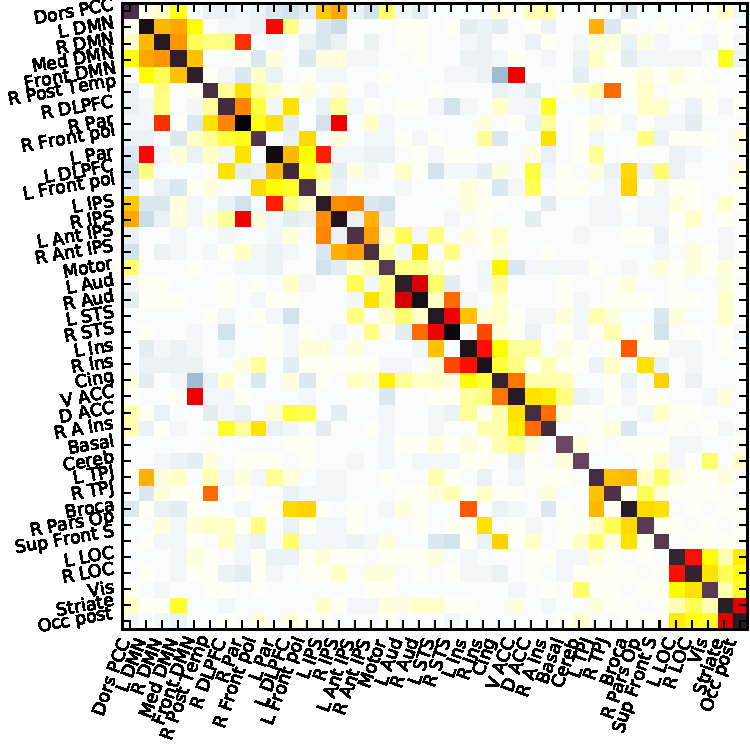
\includegraphics[width=\linewidth]{group_l21_prec.pdf}%
    \raisebox{.606\linewidth}{%
	\hspace*{-.462\linewidth}%
	\photoframe{%
	%\setlength\fboxsep{1pt}%
	\colorbox{white}{%
	\raisebox{.003\linewidth}{%
	    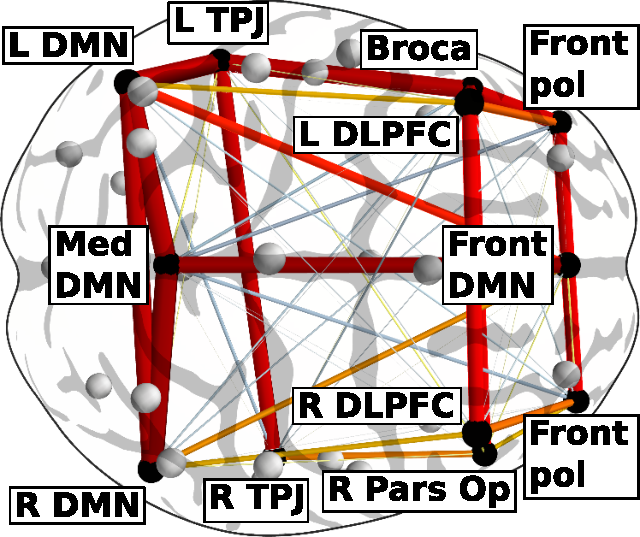
\includegraphics[width=.455\linewidth]{group_l21_prec_3d_labels}}%
	\rule{0pt}{.387\linewidth}%
	}}%
    }
\end{minipage}%
\hspace*{1pt}%
\begin{minipage}{.33\linewidth}%
    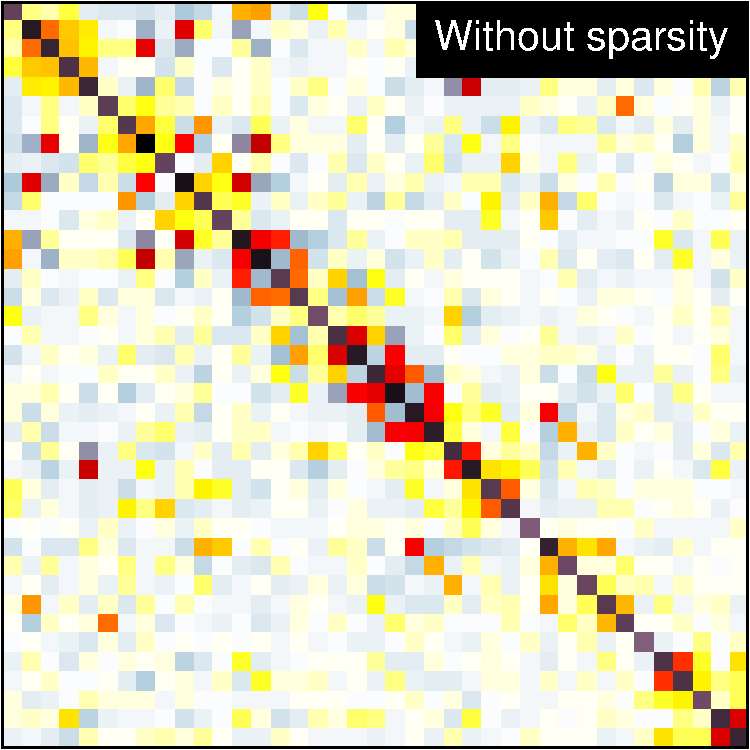
\includegraphics[width=\linewidth]{group_emp_prec.pdf}%

    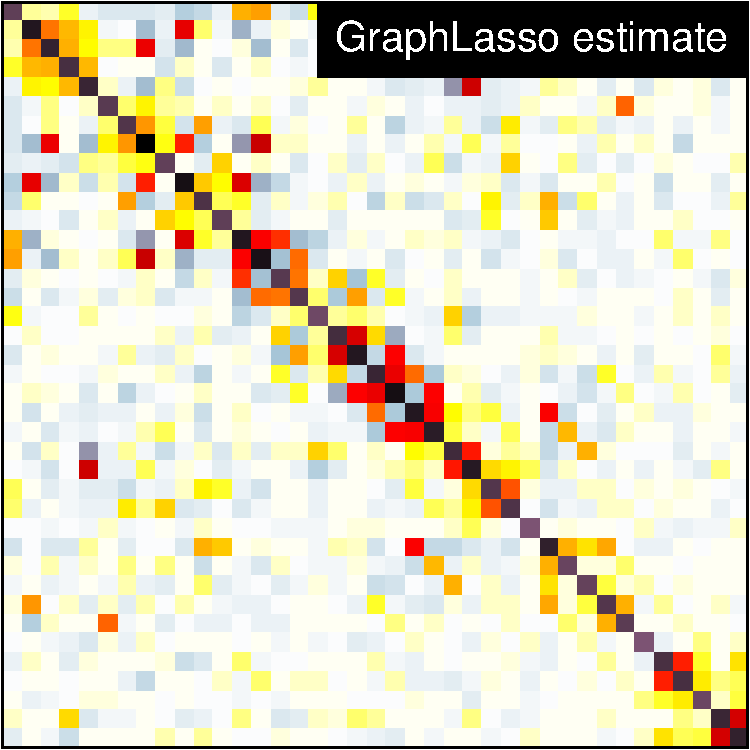
\includegraphics[width=\linewidth]{group_l1_prec.pdf}%
\end{minipage}%

\caption{
Different inverse-covariance matrices estimates corresponding to
Fig.\,\ref{fig:correlation_matrices} -- \textbf{Left}: group-sparse estimate
using the $\ell_{21}$ estimator \cite{varoquaux2010c}.
The insert shows the
connections restricted to the default mode network. -- \textbf{Upper
right}: non-sparse estimate: inverse of the sample correlation matrix. --
\textbf{Lower right}: sparse estimate using the Graph Lasso
\cite{friedman2008}.
\label{fig:icov_estimators}
}
\end{figure}
%---------------------------------------------------------------------------}}}


\paragraph{Correlation and partial correlations}
%
Functional connectivity between the ROIs can be measured by computing the
correlation matrix of the extracted signals. An important and often
neglected point is that the sample correlation matrix, \emph{i.e.}\ the
correlation matrix obtained by plugging the observed signal in the
correlation matrix formula, is not the population correlation matrix,
\emph{i.e.}\ the correlation matrix of the data-generating process. If the
number of measurements was infinite, the two would coincide, however if
this number is not large compared to the number of connection (that
scales as the square of the number of ROIs), the sample correlation
matrix is a poor estimate of the underlying population correlation
matrix. In other words, the sample correlation matrix captures a lot of
sampling noise, intrinsic randomness that arises in the estimation of
correlations from short time series. Conclusions drawn from the sample
correlation matrix can easily reflect this estimation error.
%
Varoquaux \emph{et al.}~\cite{varoquaux2010c} and Smith \emph{et
al.}~\cite{smith2011} have shown respectively on rest fMRI and on
realistic simulations that a good choice of correlation matrix estimator
could recover the connectivity structure, where the sample correlation
matrix would fail. In general, the choice of a better estimate depends on
the settings and the end goals \cite{varoquaux2012,varoquaux2010b},
however the Ledoit-Wolf shrinkage estimate \cite{ledoit2004} is a simple,
computationally-efficient, and parameter-less alternative that performs
uniformly better than the sample correlation matrix
\cite{varoquaux2012,varoquaux2010c} and should always be preferred.


%{{{------ Regressor in precision matrix -------------------------------------
\begin{figure}
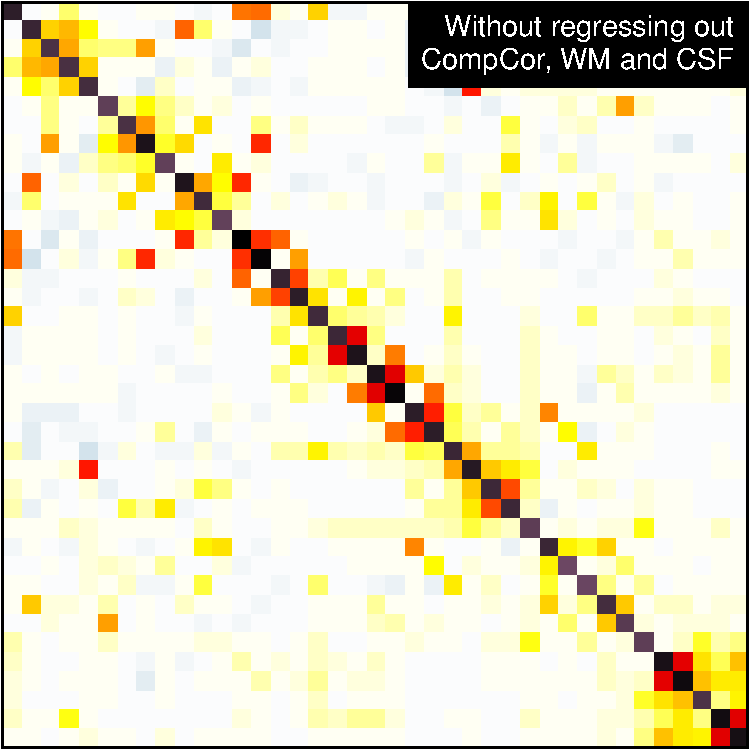
\includegraphics[height=.482\linewidth]{group_l21_prec_no_confounds.pdf}%
\hspace*{1pt}%
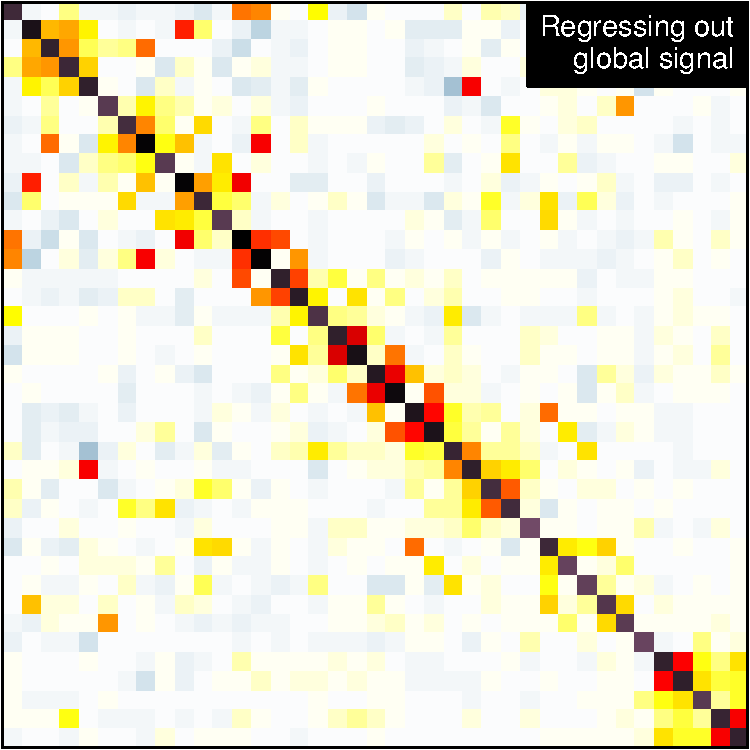
\includegraphics[height=.482\linewidth]{group_l21_prec_global_mean.pdf}%
\hspace*{1pt}%

\includegraphics[height=.482\linewidth]{cmap.pdf}%

\caption{Inverse covariance matrices for different choice of
confound regressors --
\label{fig:icov_regressors}
\textbf{Left}: regressing out only movement parameters --
\textbf{Right}: removal of the global mean,
instead of the white matter, CSF, and CompCor time courses. 
}
\end{figure}
%---------------------------------------------------------------------------}}}



For the problem of recovering the functional-connectivity
\emph{structure}, \emph{i.e.}\ finding which region is connected to
which, sparse inverse covariance estimators have been found to be
efficient \cite{varoquaux2010c, smith2011}. The intuition for relying on
inverse covariance rather than correlation stems from that fact that
standard correlation (marginal correlation) between two variables $a$ and
$b$ also capture the effects of other variables -- strong correlation of
$a$ and $b$ with a third variable $c$ will induce a correlation between
$a$ and $b$. On the opposite, the inverse covariance\footnote{Covariance
and correlation matrices differ simply by the fact that a covariance
matrix captures the amplitude of a signal, via its variance, while a
correlation matrix is computed on normalized signals.}
matrix captures
partial correlations, removing the effect of other variables
\cite{marrelec2006a}. In the small sample limit, this removal is
challenging from the statistical standpoint, and assumption of sparsity,
\emph{i.e.}\ that only few variables need to be considered at a time, is
important to estimate a good inverse covariance. Various estimation
strategies exist for sparse inverse covariance, and have an impact on the
resulting networks \cite{varoquaux2012,varoquaux2010c}. The
Graph Lasso ($\ell_1$-penalized maximum-likelihood estimator)
\cite{friedman2008} is in general a good approach for structure recovery. In group studies,
the $\ell_{21}$ estimator \cite{varoquaux2010c,honorio2012} is useful to
impose a common sparsity structure across different subjects and achieve
better recovery of this common structure. Simply put, these approaches
are necessary because estimation noise creates a background structure
(see Fig.\,\ref{fig:icov_estimators}); however, unlike in a univariate situation, the
parameters are not independent, and the spurious background connections
degrade the estimation of the actual connections. The sparse estimators
make a compromise between imposing simpler models, \emph{i.e.}\ with less
connections, and fitting well the data. This compromise is set via a
regularization parameter which controls the sparsity of the estimate. A
good rule of thumb to set this parameter is via cross-validation
\cite{varoquaux2010c}.

% XXX: must comment on the estimator figure

\paragraph{Network structure extracted}
%
The correlation matrices and inverse-covariance matrices that we extract
contain a lot of information on the functional structure of the brain.
First, the correlation matrix (Fig.\,\ref{fig:correlation_matrices})
shows blocks of coactivating regions that can be interpreted as
large-scale functional networks, such as the default mode network. Note
the split in network is not straightforward. Different ordering of the
nodes will reveal different networks. Indeed, because of the presence of
hubs and interleaved networks the picture in terms of segregated networks
is not sufficient to explain full-brain connectivity
\cite{varoquaux2012}. The connectivity matrices, correlation matrix or
inverse-covariance matrix, can be represented as graphs: nodes connected
by weighted edges (inserts on Fig.\,\ref{fig:correlation_matrices} and
Fig.\,\ref{fig:icov_estimators}). The inverse-covariance matrix,
capturing partial correlations, appears then as extracting a
\emph{backbone} or \emph{core} of the graph. While such structure have
been used as a way to summarize anatomical brain connectivity graphs
\cite{hagmann2008}, here they have a clear-cut meaning with regards to
the BOLD signal: they give the conditional independence structure between
the regions \cite{varoquaux2012}. In other words, regions $a$ and $b$ are
not connected if the signal that they have in common can be explained by
a third region $c$. In this light, the choice of nuisance regressors to
remove confounding common signal is less critical. Indeed, while with
correlation matrices regressing out the global mean has a drastic
(Fig.\,\ref{fig:correlation_matrices} upper right and lower right), on
inverse covariance it only changes very slightly the resulting matrices
(Fig.\,\ref{fig:icov_regressors}). There have been debates on whether to
regress out certain signals, such as the global mean,  as it induces
negative correlations \cite{murphy2009,chang2009,fox2009}, and these may seem
surprising: one network is doing the opposite of the other. However,
correlation between two signals only takes its meaning with the
definition of a baseline. A simple picture to explain anti-correlations
between two regions is the presence of a third region, mediating the
interactions. Using this third region as a baseline would amount to
estimate partial correlations in the whole system. Using 
inverse-covariance matrices or partial correlations to understand brain
connectivity makes the interpretation in terms of interactions between
brain regions easier and more robust to the choice of confounds.

% XXX: where to insert this in the above paragraph: cite the
% Fransson/Marrelec paper on the role of the PCC

% \cite{chai2011} (note: chai2011 used compcor)
% Remark that partial correlations consistently have no negative values.


%%%%%%%%%%%%%%%%%%%%%%%%%%%%%%%%%%%%%%%%%%%%%%%%%%%%%%%%%%%%%%%%%%%%%%%%%%%%%%%

\section{Comparing connectivity}

Here, we consider the problem of comparing functional connectivity across
subjects or across conditions.

%------------------------------------------------------------------------------
\subsection{Detecting changing connections}

First, we focus on detecting where the connectivity matrices estimated in
the previous section differ. \paragraph{Mass-univariate approaches}
%
The most natural approach is to do a linear model on each coefficient of
the connectivity matrices, as in \cite{lewis2009,grillon2012}. This
approach is similar to the second-level analysis used in mass-univariate
brain mapping, and will give rise to many of the well-known techniques
used in such a context, such as the definition of second-level design,
with possibly the inclusion of confounding effects, and statistical tests
(T tests or F tests) on contrast vector. Importantly, in order to work
with Gaussian-distributed correlations, it is necessary to apply a Fisher
Z transform\footnote{See
\url{http://en.wikipedia.org/wiki/Fisher_transformation} or
\cite{anderson1958}, section 4.2.3 for mathematical arguments}. Note that
in these settings, the Ledoit-Wolf estimator \cite{ledoit2004} is
probably a good choice to estimate the correlation matrix, as it is
parameter-less and gives good estimation performance without imposing any
restrictions on the data.
%
Correcting for multiple comparison can often severely limit statistical
power, as the number of tests performed scales as the square of the
number of regions used. Controlling for the false discovery rate (FDR)
mitigates this problem. Alternatively, as the assumption underlying the
Benjamini-Hochberg procedure \cite{benjamini1995} for the FDR can easily
be broken, non-parametric permutations-based approaches give reliable
approaches. In particular, the max-T procedure \cite{ge2003,nichols2001}
is interesting to avoid the drastic Bonferroni correction when
controlling for multiple comparison in family-wise error rate.

%{{{------ Inter subject fluctuations ----------------------------------------
\begin{figure}
\hspace*{.5ex}%
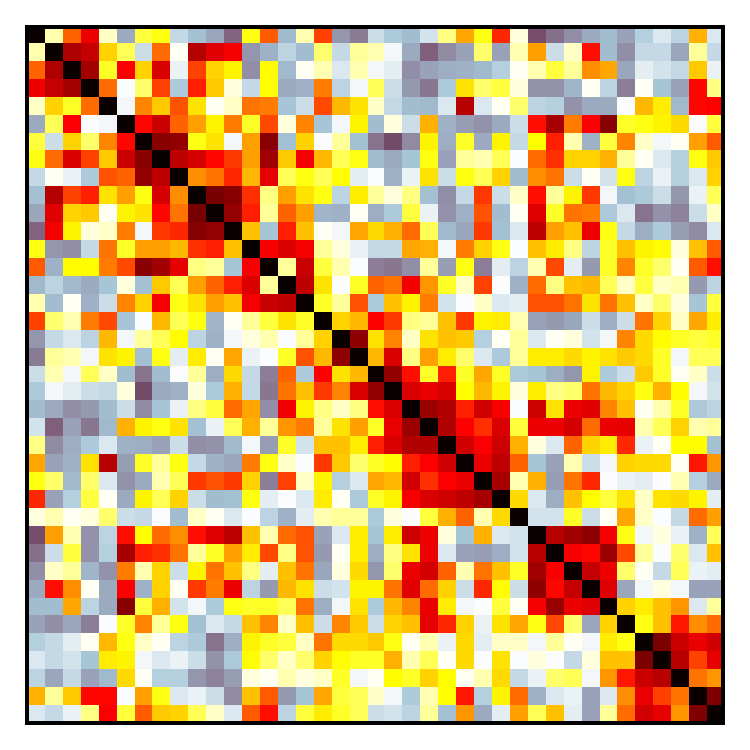
\includegraphics[width=.196\linewidth]{inter_subj/cov_sub00.pdf}%
\hspace*{-.2ex}%
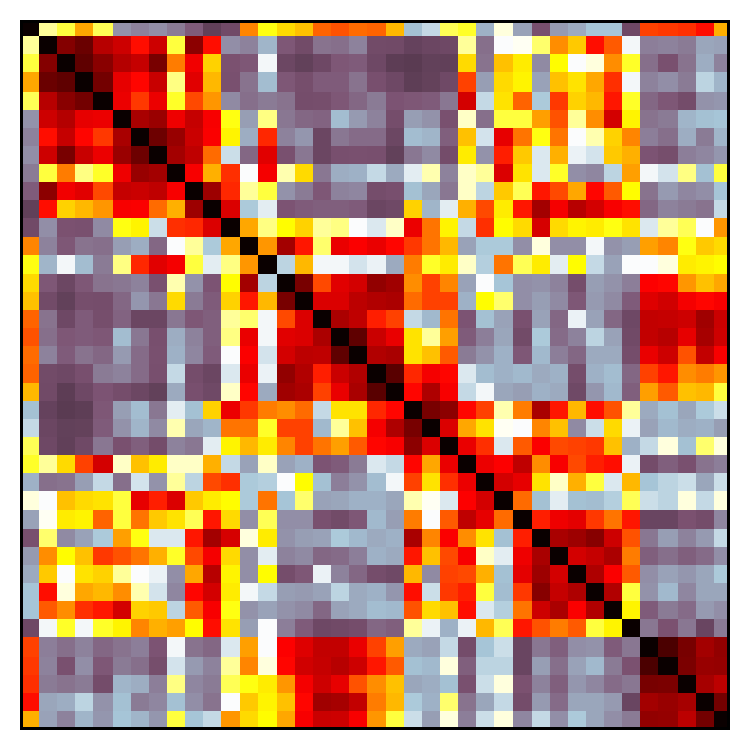
\includegraphics[width=.196\linewidth]{inter_subj/cov_sub29.pdf}%
\hspace*{-.2ex}%
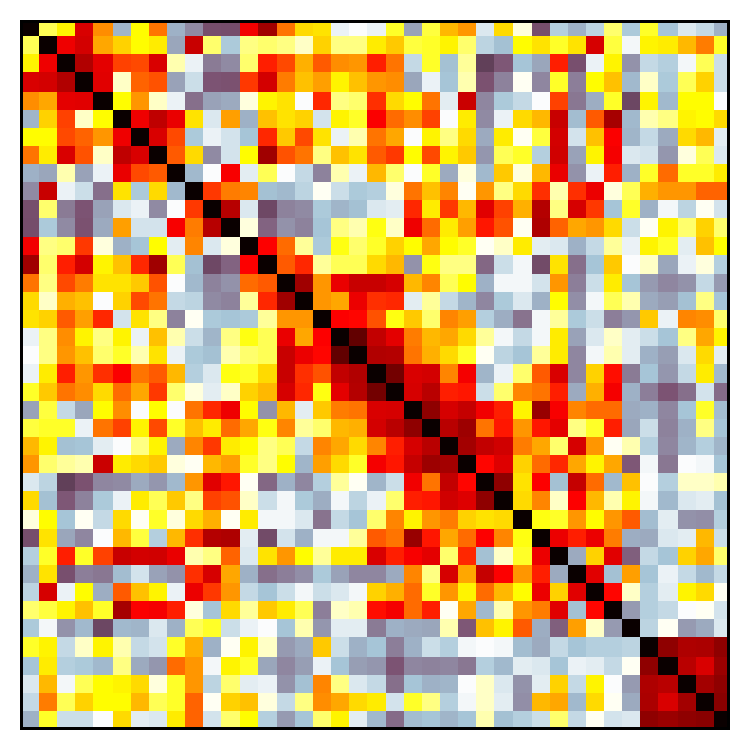
\includegraphics[width=.196\linewidth]{inter_subj/cov_sub01.pdf}%
\hspace*{-.2ex}%
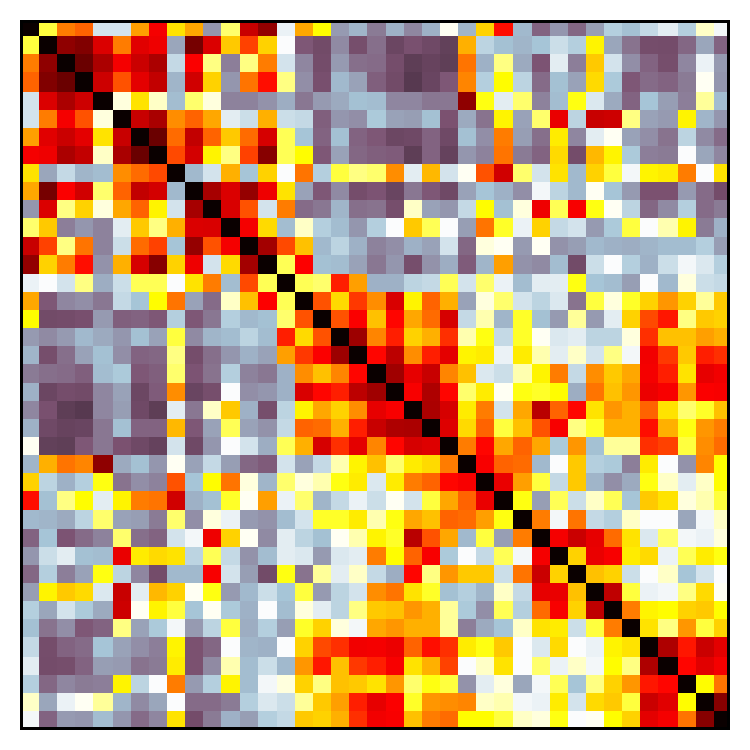
\includegraphics[width=.196\linewidth]{inter_subj/cov_sub07.pdf}%
\hspace*{-.2ex}%
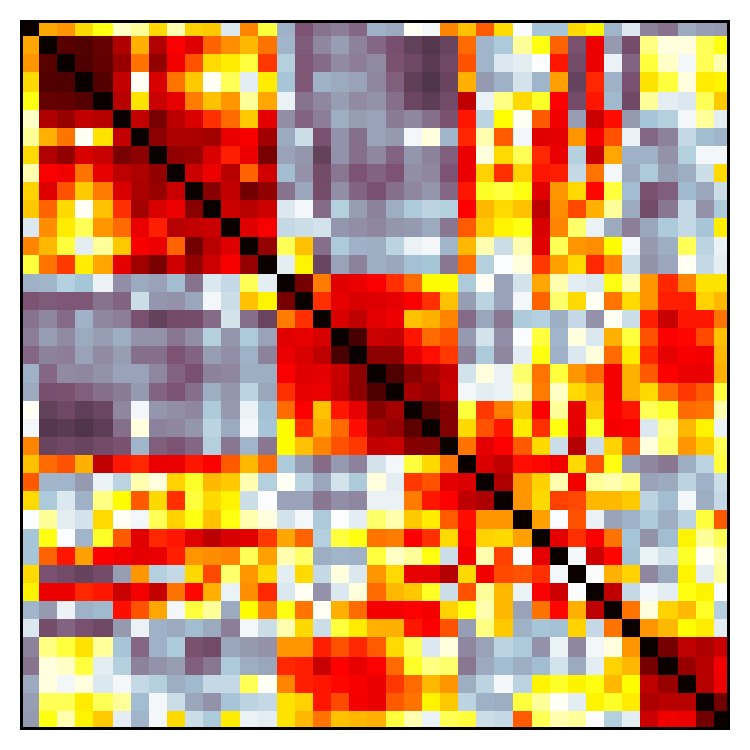
\includegraphics[width=.196\linewidth]{inter_subj/cov_sub53.pdf}%
\hspace*{.1ex}%
\raisebox{.005\linewidth}{%
    
\includegraphics[width=.0186\linewidth]{cmap_00.pdf}%
    \llap{
	\raisebox{.003\linewidth}{%
	    \bfseries\tiny\color{white} -\!1\hspace*{-.2ex}}%
    }%
    \llap{
	\raisebox{.17\linewidth}{%
	    \bfseries\tiny\color{white} 1\hspace*{.1ex}}%
    }%
}%
\llap{\rlap{
    \setlength\fboxsep{1pt}%
    \raisebox{.16\linewidth}{%
	\colorbox{black!10}{%
	    \sffamily\small\textbf{a}. Correlation matrices}}%
	}%
    \hspace*{.993\linewidth}%
}


\hspace*{.5ex}%
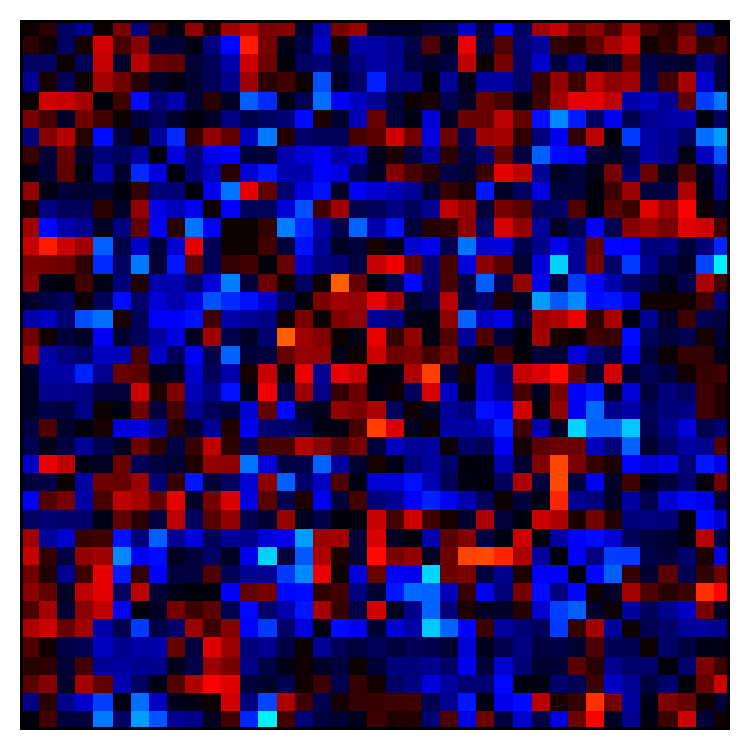
\includegraphics[width=.196\linewidth]{inter_subj/z_score_sub00.pdf}%
\hspace*{-.2ex}%
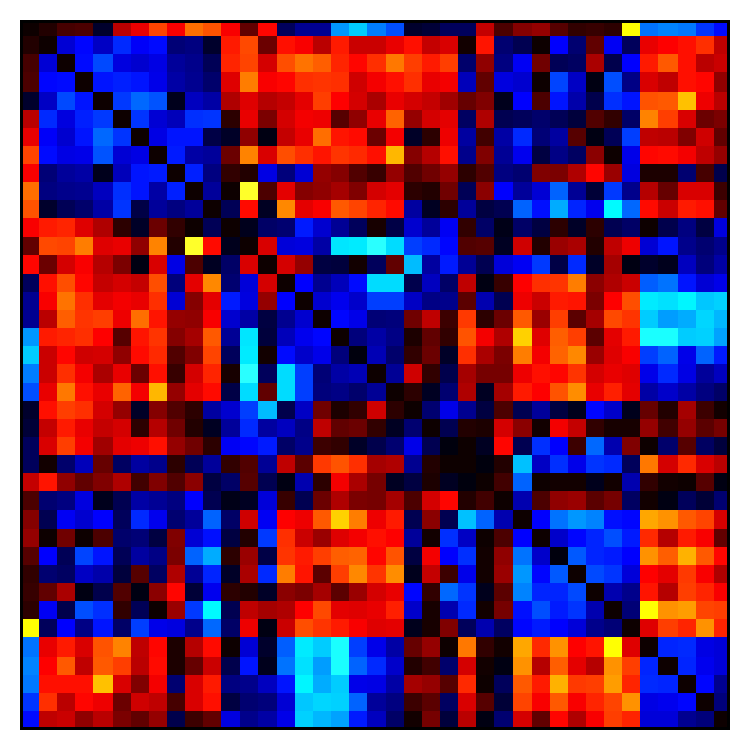
\includegraphics[width=.196\linewidth]{inter_subj/z_score_sub29.pdf}%
\hspace*{-.2ex}%
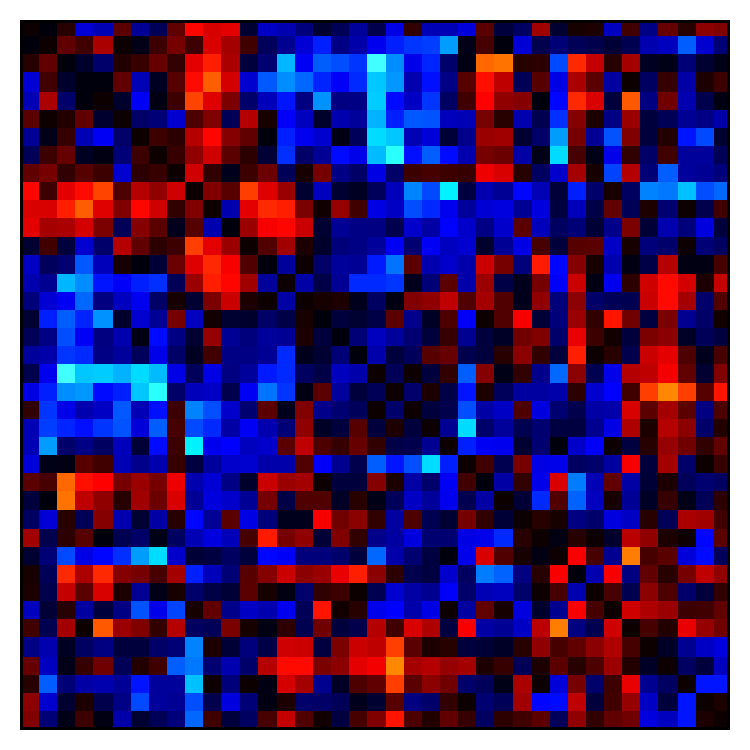
\includegraphics[width=.196\linewidth]{inter_subj/z_score_sub01.pdf}%
\hspace*{-.2ex}%
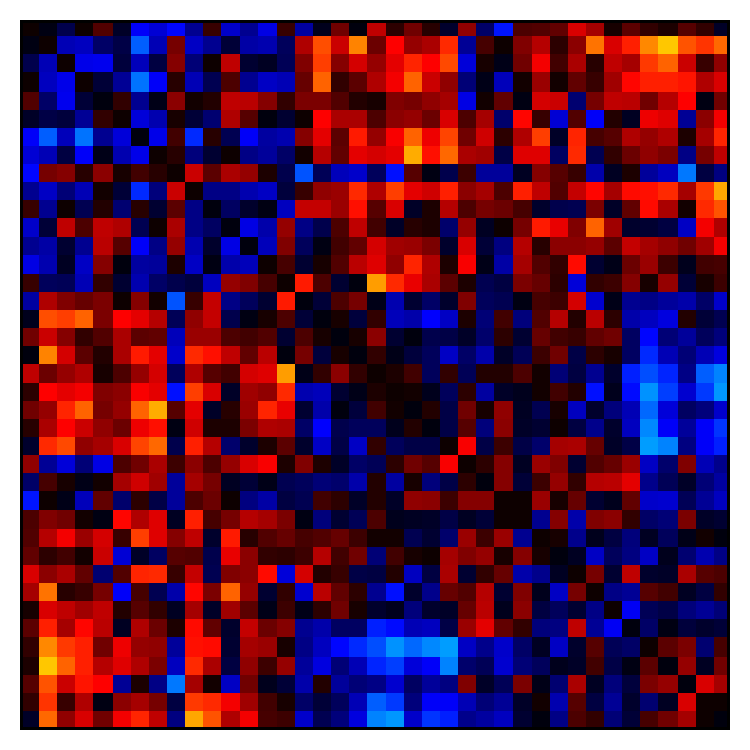
\includegraphics[width=.196\linewidth]{inter_subj/z_score_sub07.pdf}%
\hspace*{-.2ex}%
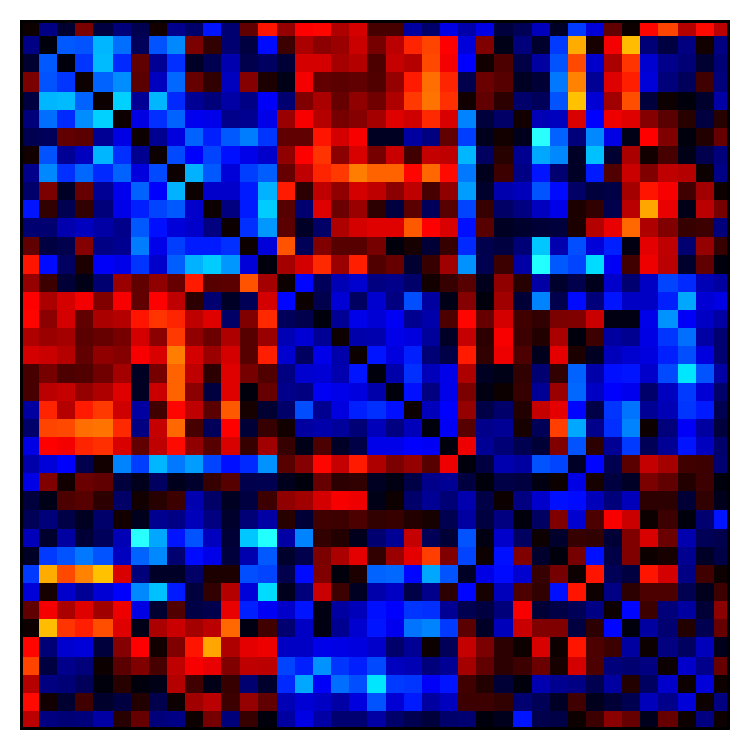
\includegraphics[width=.196\linewidth]{inter_subj/z_score_sub53.pdf}%
\hspace*{.1ex}%
\raisebox{.005\linewidth}{%
    
\includegraphics[width=.0186\linewidth]{cmap_01.pdf}%
    \llap{
	\raisebox{.003\linewidth}{%
	    \bfseries\tiny -\!\hspace*{-.1ex}4\hspace*{-.1ex}}%
    }%
    \llap{
	\raisebox{.168\linewidth}{%
	    \bfseries\tiny 4\hspace*{.1ex}}%
    }%
}%
\llap{\rlap{
    \setlength\fboxsep{1pt}%
    \raisebox{.16\linewidth}{%
	\colorbox{black!10}{%
	    \sffamily\small\textbf{b}. Z score on difference}}%
	}%
    \hspace*{.993\linewidth}%
}

\hspace*{.5ex}%
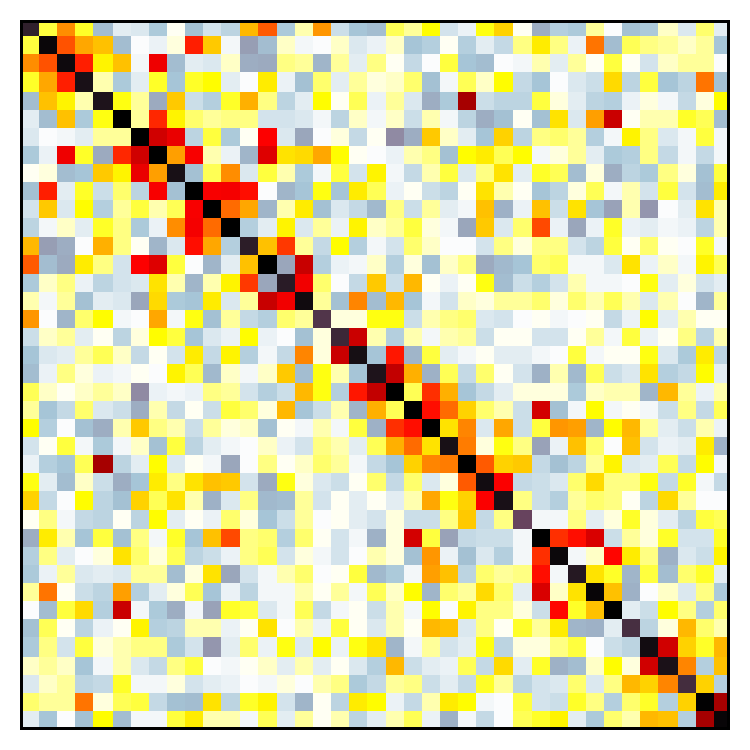
\includegraphics[width=.196\linewidth]{inter_subj/prec_sub00.pdf}%
\hspace*{-.2ex}%
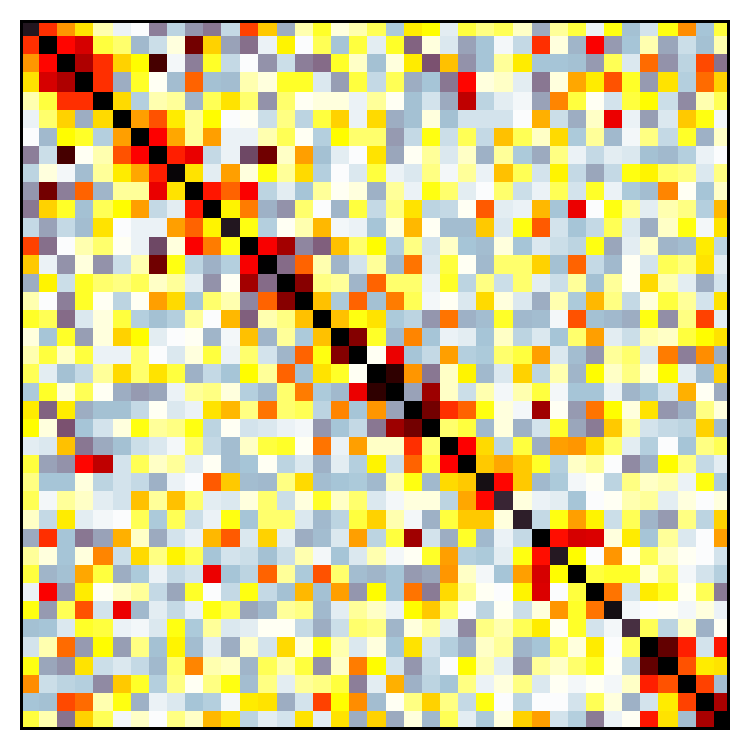
\includegraphics[width=.196\linewidth]{inter_subj/prec_sub29.pdf}%
\hspace*{-.2ex}%
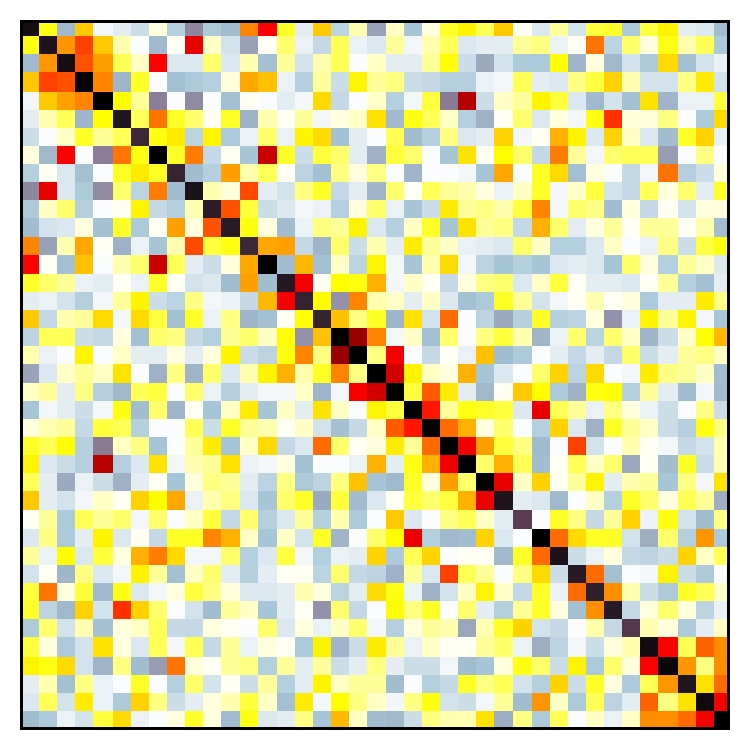
\includegraphics[width=.196\linewidth]{inter_subj/prec_sub01.pdf}%
\hspace*{-.2ex}%
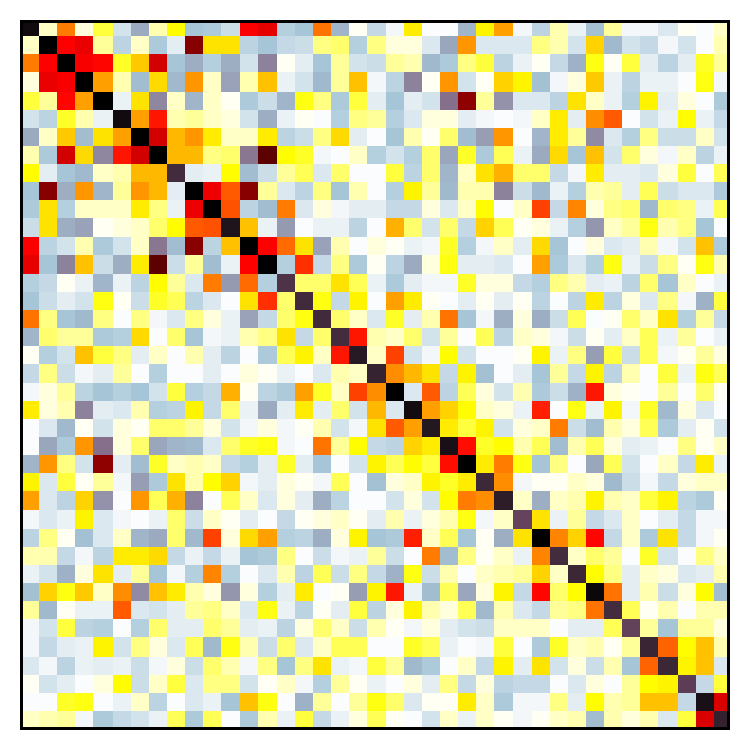
\includegraphics[width=.196\linewidth]{inter_subj/prec_sub07.pdf}%
\hspace*{-.2ex}%
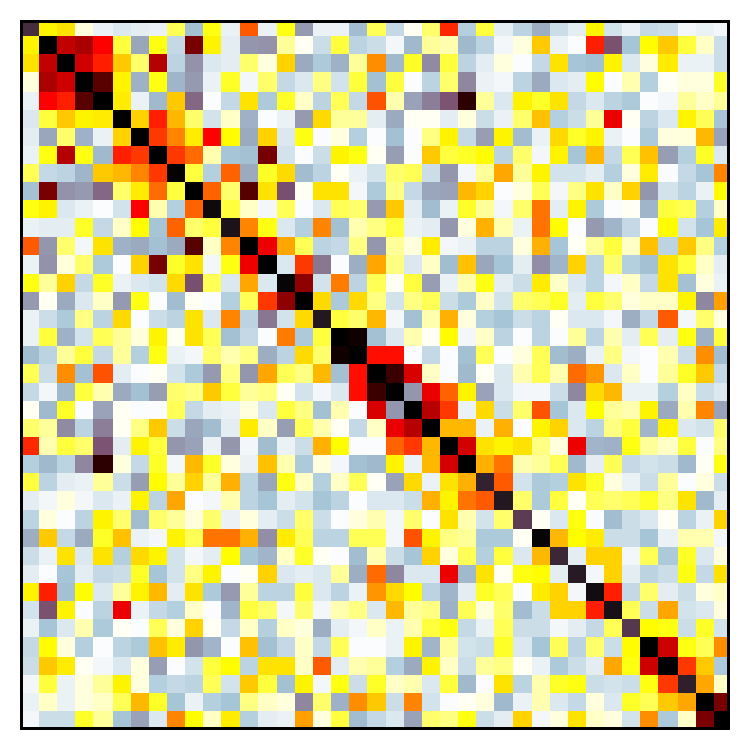
\includegraphics[width=.196\linewidth]{inter_subj/prec_sub53.pdf}%
\hspace*{.1ex}%
\raisebox{.005\linewidth}{%
    
\includegraphics[width=.0186\linewidth]{cmap_00.pdf}%
    \llap{
	\raisebox{.003\linewidth}{%
	    \bfseries\tiny\color{white} -\!1\hspace*{-.2ex}}%
    }%
    \llap{
	\raisebox{.17\linewidth}{%
	    \bfseries\tiny\color{white} 1\hspace*{.1ex}}%
    }%
}%
\llap{\rlap{
    \setlength\fboxsep{1pt}%
    \raisebox{.16\linewidth}{%
	\colorbox{black!10}{%
	    \sffamily\small\textbf{c}. Inverse-covariance matrices}}%
	}%
    \hspace*{.993\linewidth}%
}

\hspace*{.5ex}%
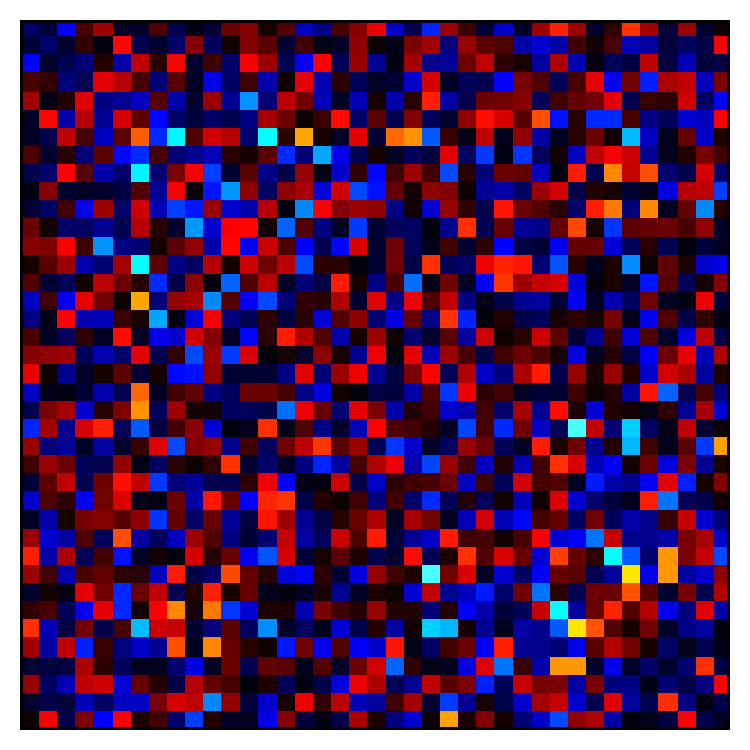
\includegraphics[width=.196\linewidth]{inter_subj/z_score_prec_sub00.pdf}%
\hspace*{-.2ex}%
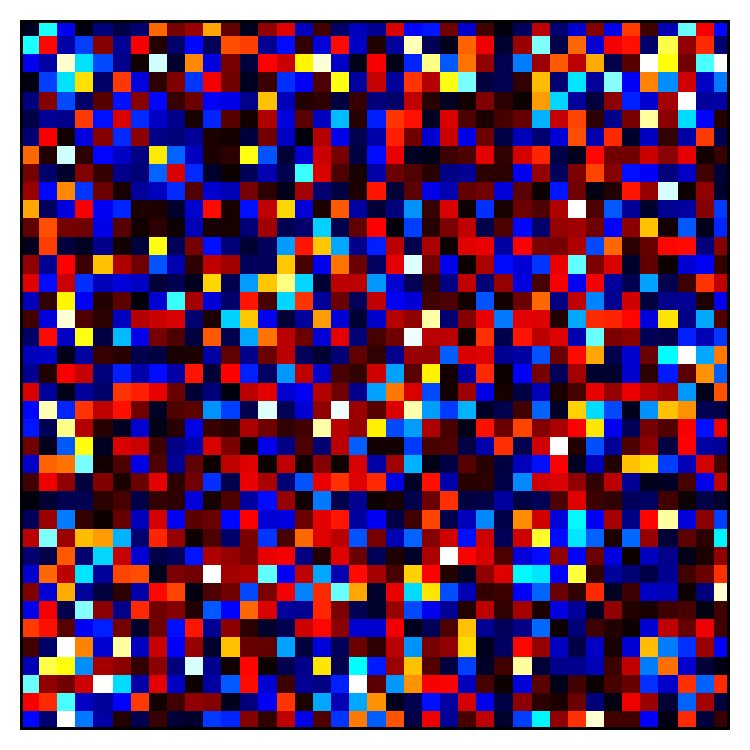
\includegraphics[width=.196\linewidth]{inter_subj/z_score_prec_sub29.pdf}%
\hspace*{-.2ex}%
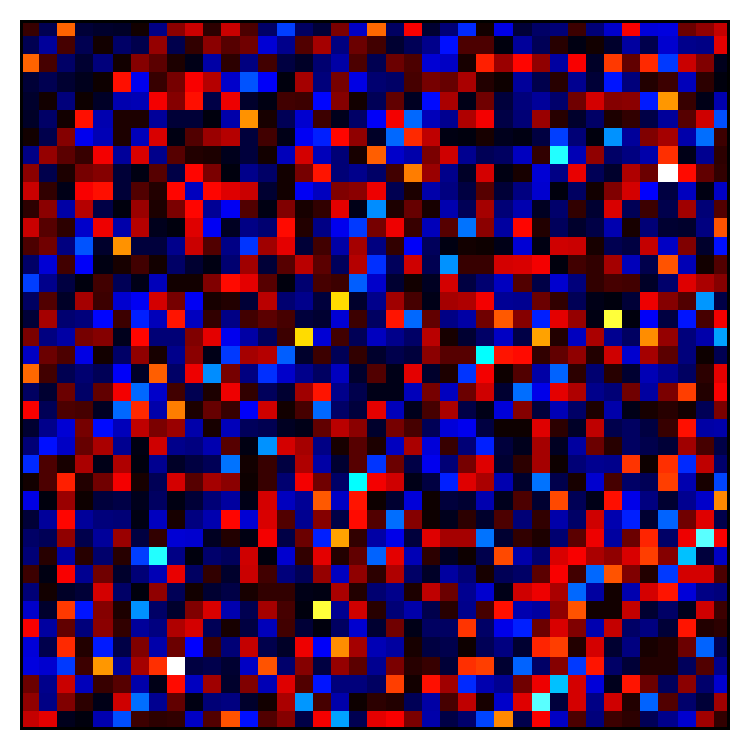
\includegraphics[width=.196\linewidth]{inter_subj/z_score_prec_sub01.pdf}%
\hspace*{-.2ex}%
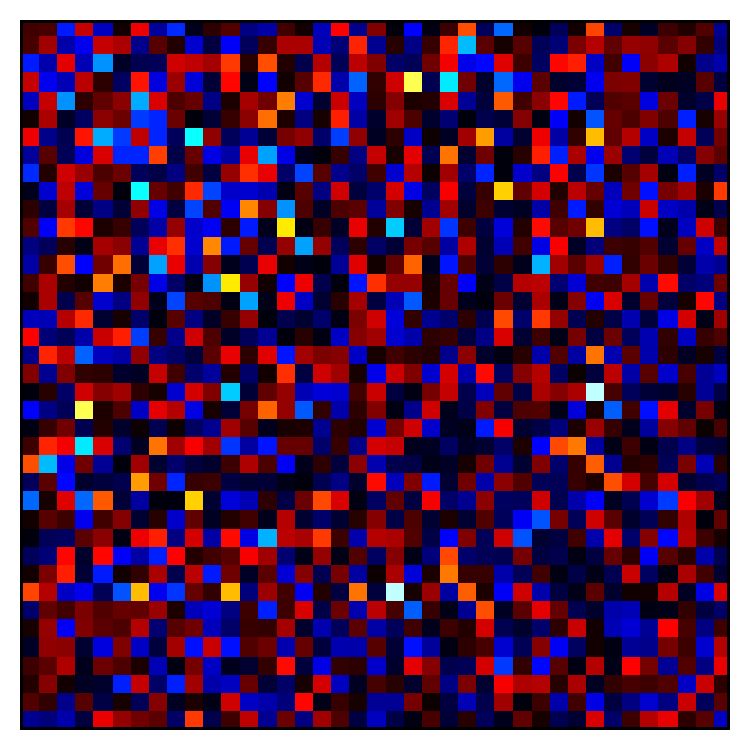
\includegraphics[width=.196\linewidth]{inter_subj/z_score_prec_sub07.pdf}%
\hspace*{-.2ex}%
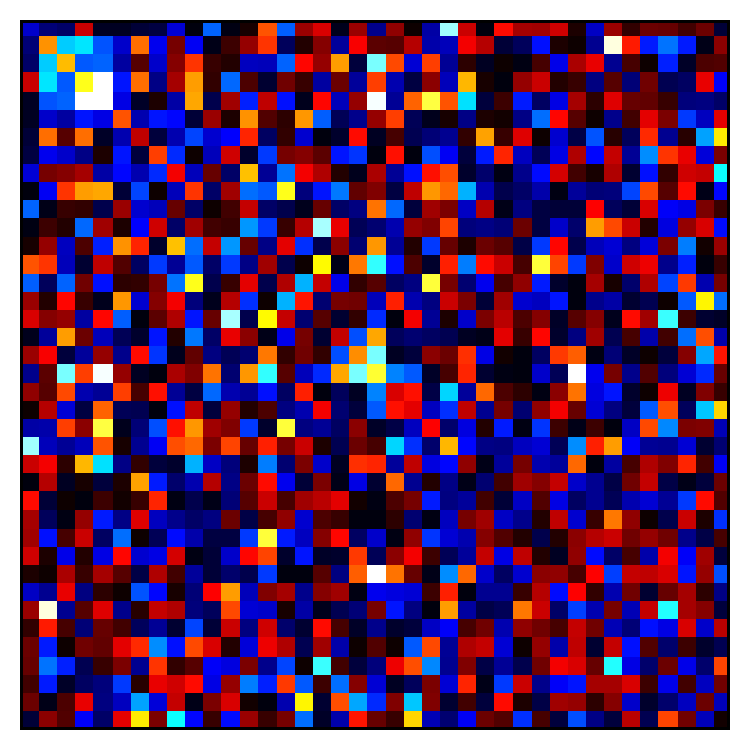
\includegraphics[width=.196\linewidth]{inter_subj/z_score_prec_sub53.pdf}%
\hspace*{.1ex}%
\raisebox{.005\linewidth}{%
    
\includegraphics[width=.0186\linewidth]{cmap_01.pdf}%
    \llap{
	\raisebox{.003\linewidth}{%
	    \bfseries\tiny -\!\hspace*{-.1ex}4\hspace*{-.1ex}}%
    }%
    \llap{
	\raisebox{.168\linewidth}{%
	    \bfseries\tiny 4\hspace*{.1ex}}%
    }%
}%
\llap{\rlap{
    \setlength\fboxsep{1pt}%
    \raisebox{.16\linewidth}{%
	\colorbox{black!10}{%
	    \sffamily\small\textbf{d}. Z score on inverse-covariance}}%
	}%
    \hspace*{.993\linewidth}%
}



\hspace*{.5ex}%
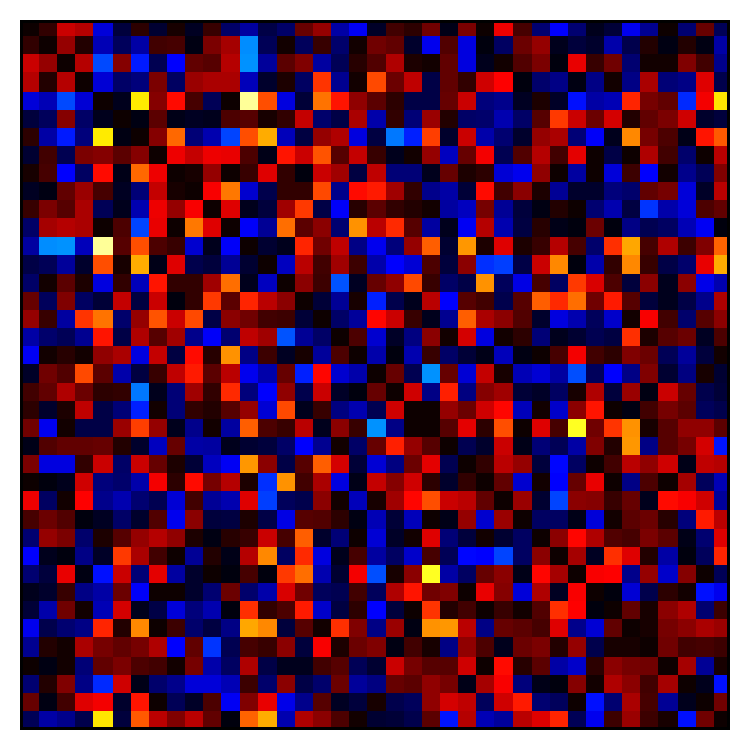
\includegraphics[width=.196\linewidth]{inter_subj/res_sub00.pdf}%
\hspace*{-.2ex}%
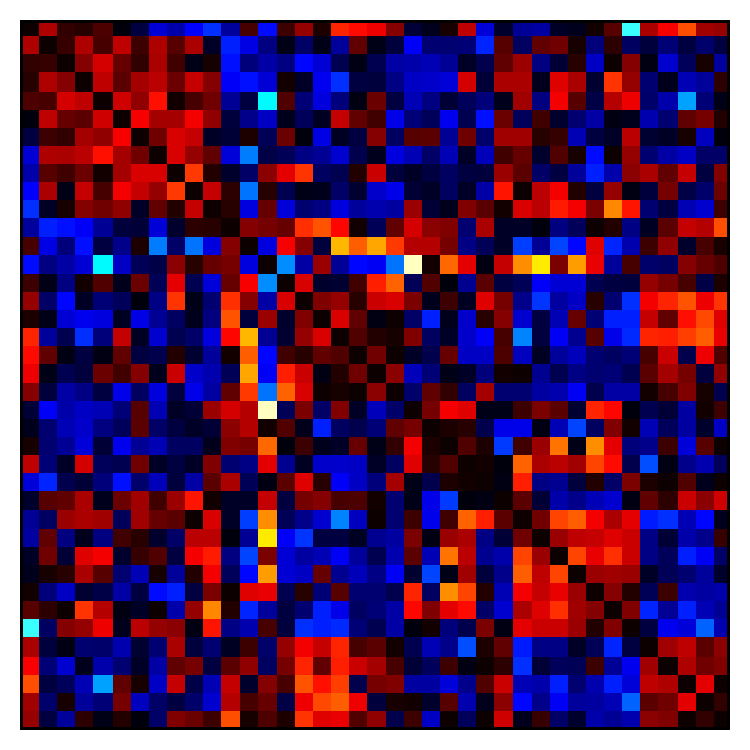
\includegraphics[width=.196\linewidth]{inter_subj/res_sub29.pdf}%
\hspace*{-.2ex}%
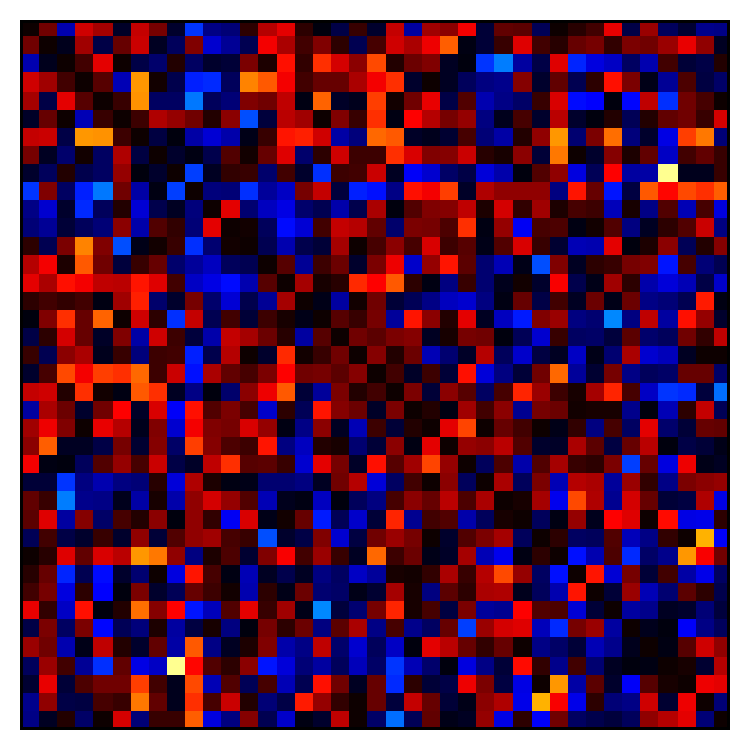
\includegraphics[width=.196\linewidth]{inter_subj/res_sub01.pdf}%
\hspace*{-.2ex}%
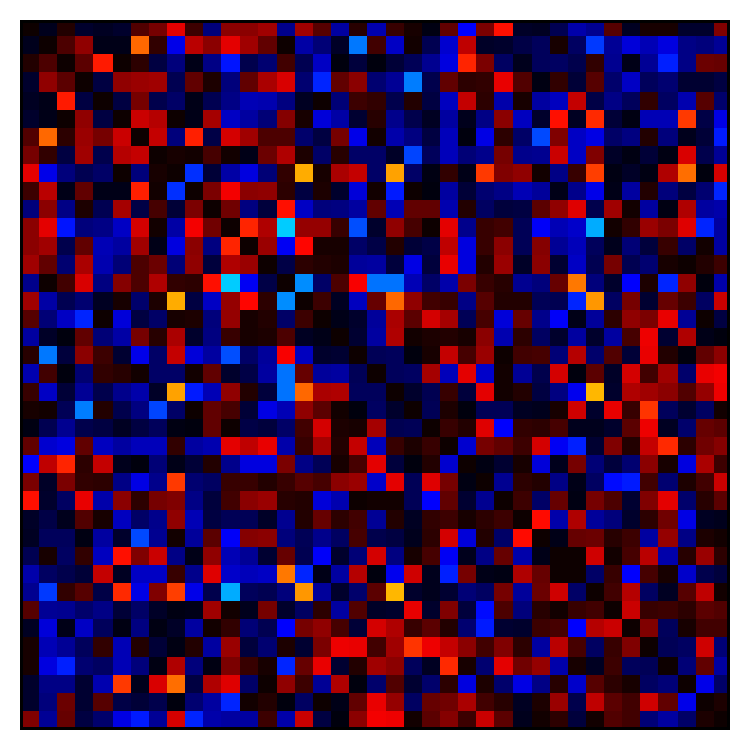
\includegraphics[width=.196\linewidth]{inter_subj/res_sub07.pdf}%
\hspace*{-.2ex}%
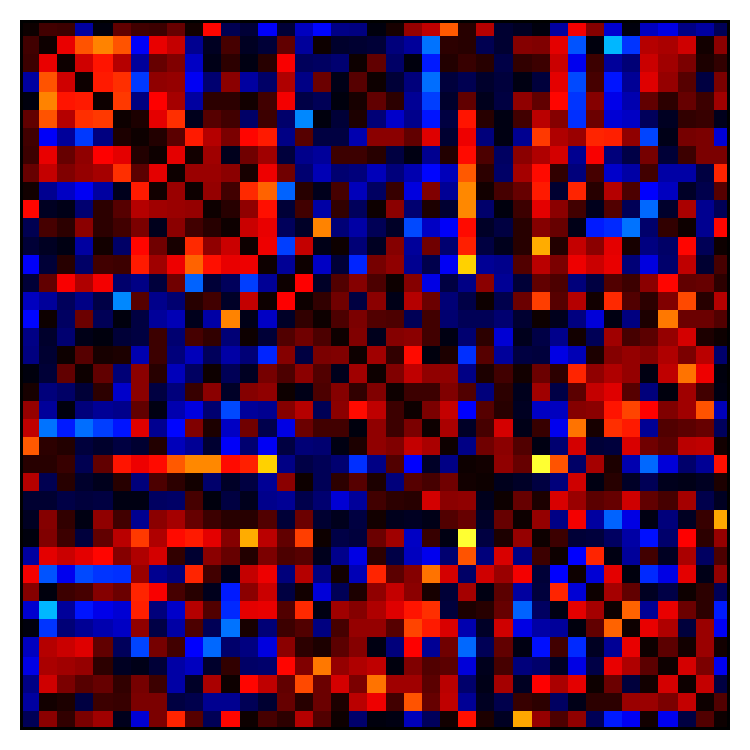
\includegraphics[width=.196\linewidth]{inter_subj/res_sub53.pdf}%
\hspace*{.1ex}%
\raisebox{.005\linewidth}{%
    
\includegraphics[width=.0186\linewidth]{cmap_01.pdf}%
    \llap{
	\raisebox{.003\linewidth}{%
	    \bfseries\tiny -\!\hspace*{-.1ex}4\hspace*{-.1ex}}%
    }%
    \llap{
	\raisebox{.168\linewidth}{%
	    \bfseries\tiny 4\hspace*{.1ex}}%
    }%
}%
\llap{\rlap{
    \setlength\fboxsep{1pt}%
    \raisebox{.16\linewidth}{%
	\colorbox{black!10}{%
	    \sffamily\small\textbf{e}. Z score on residuals \scriptsize
		\raisebox{.2ex}{\cite{varoquaux2010b}}}}%
	}%
    \hspace*{.993\linewidth}%
}

\caption{Inter subject variability. Note that this is variability
occurring in a healthy population at rest, in other words non specific
variability -- \textbf{a}: single-subject
correlation matrices for different subjects -- \textbf{b}:
Corresponding Z-score (effect / standard deviation) of the difference
between a subject and the remaining others -- \textbf{c}:
single-subject precision matrices -- \textbf{d}: Corresponding Z-score
for the precision matrices -- \textbf{e}:
Corresponding Z-score for the subject residuals, as defined in 
\cite{varoquaux2010b}.
\label{fig:inter_subject}}
\end{figure}
%---------------------------------------------------------------------------}}}

\paragraph{Accounting for distributed variability}
%
A specific challenge of connectivity analysis is that the connectivity
between different regions tend to covary. For instance, with
resting-state data, functional networks comprising many nodes can appear
as more or less connected across subjects (see for instance
Fig.\,\ref{fig:inter_subject}.a, showing variability in a control
population at rest). In other words, non-specific variability is
distributed accross the connectivity graph, and it is structured by the
graph itself. This observation brings the natural question of whether
second-level analysis should be performed on correlation matrices,
inverse-covariance matrices, or another parametrisation that would
disentangle effects and give unstructured (white) residuals. While
inverse-covariance matrices show less distributed fluctuations than
correlation matrices, they capture a lot of background noise, as partial
correlations are intrinsically harder to estimate. Preliminary work
\cite{varoquaux2010b} suggest to perform statistics on residuals of
a parametrisation intermediate between correlation matrix and inverse
covariance matrix.

Taking a different stance on distributed variability, the ``network-based
statistics'' approach \cite{zalesky2010} draws from the hypothesis that
if, in a second-level analysis, an effect is detected in a connection
that lies in a network of strongly connected nodes, the whole network is
likely to cary an effect. Thus, they adapt cluster-level inference to
connectivity analysis, in order to mitigate the curse of multiple
comparisons.

%------------------------------------------------------------------------------

\subsection{Comparing network summary statistics}

\paragraph{Network integration}
%
To avoid the multiple comparison issue and to capture the network-level
distributed variability, a possible strategy is to perform comparison and
statistical testing at the level of the network, rather than the
individual connection. In particular, Marrelec \emph{et al.}\
\cite{marrelec2008} introduce the use of entropy and mutual information
as a measure of network integration\footnote{See \cite{varoquaux2010c}
for simplified formulas for network integration and mutual information.}.
Gaussian entropy can be seen as a simple metric to generalize correlation
or variance to multiple nodes (see \cite{anderson1958} \S2.5.2 and
\S7.5). Indeed, let us considering 3 nodes: $a$, $b$ and $c$. Their
correlation structure is captured by three correlation coefficients:
$\rho_{ab}$, $\rho_{bc}$ and $\rho_{ac}$. Summarizing these by their
mean, as it might seem natural, discards the relationship between the
signals, while using the integration tells us how much two signals can be
combined to form the third (see Fig.\,\ref{fig:integration}). Similarly
as Gaussian entropy can be used to measure the integration of a brain
system or network, cross-entropy --or mutual information--
\cite{marrelec2008} measures the amount of cross-talk between two
systems. The functional-connectivity structure, or its representation in
form of a correlation matrix, can thus be characterized via the
integration and cross-talk of some of its subs-systems. This appraoch
gives a simplified representation with a small number of metrics that can
be compared across subjects.


%{{{------ Integration measure -----------------------------------------------
\begin{figure}
\hspace*{2ex}%
\begin{minipage}{.19\linewidth}
    \center\sffamily
    {\small Integration:}

    0.554
\end{minipage}%
\begin{minipage}{.2\linewidth}
    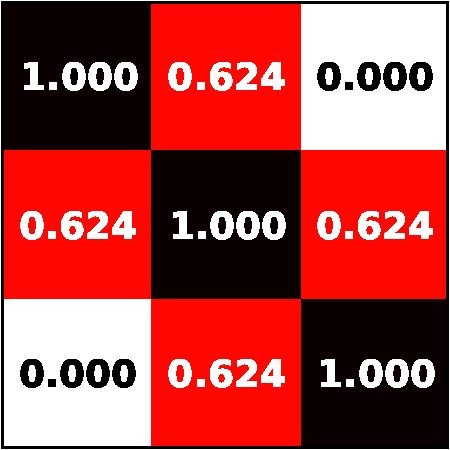
\includegraphics[width=\linewidth]{correlation_ex1.pdf}
\end{minipage}%
\hfill%
\begin{minipage}{.033\linewidth}
    
\includegraphics[width=\linewidth]{correlation_cmap.pdf}%
    \llap{\raisebox{.4ex}{\scriptsize\sffamily\bfseries 0}\hspace*{.54ex}}%
    \llap{\raisebox{10.1ex}{\scriptsize\sffamily\bfseries\color{white} 1}%
	    \hspace*{.54ex}}
\end{minipage}%
\hfill%
\begin{minipage}{.2\linewidth}
    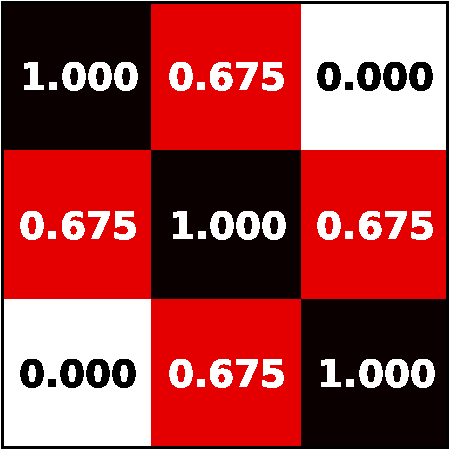
\includegraphics[width=\linewidth]{correlation_ex2.pdf}
\end{minipage}%
\begin{minipage}{.19\linewidth}
    \center\sffamily
    {\small Integration:}

    2.422
\end{minipage}%
\hspace*{2ex}%

\caption{Two different correlation matrices with the same average
correlation, but with very different integration values. Indeed, the
matrix on the left was chosen to have represent three signals $a$, $b$
and $c$ as different from each other as possible, given $\rho_{ab} +
\rho_{bc} + \rho{ac} = 1.35$; it thus as a small integration value. On
the opposite, for the matrix on the right, signal $b$ can almost be fully
recovered by combining signals $a$ and $c$; the matrix thus has a large
integration value.
\label{fig:integration}}
% Rmq: in this example, in the second figure, the 3 signals are more
% independent, and thus define a wider range of acceptable signal.
\end{figure}
%---------------------------------------------------------------------------}}}


\paragraph{Graph-topology metrics}
%
Functional connectivity graphs have been found to display specific
topological properties\footnote{In the neuroscience world, these
descriptions are group under the terms of ``graph theoretical
approaches'', however graph theory is an entire division of mathematics
and computer science that is concerned with much more than topology of
random graphs.} that are characteristic of small-word networks
\cite{stam2004,salvador2005,achard2006,bullmore2009}. These networks
display excellent transport properties: although they display relatively
small number of connections, any two regions of the brain are well
connected. Another interesting consequence of their specific topology is
the resilience it gives to the system to attacks such as resulting from
brain lesions \cite{achard2006}. This overall structure of
functional-connectivity graphs can be summarized by a few metrics, such
as the average path length between any two nodes or the local clustering
coefficients \cite{rubinov2010}. Given that pathologies without a well-defined focus, such
as schizophrenia, are thought to have a global impact on brain
connectivity \cite{liu2008,bassett2008}, it is interesting to use the
graph-topology metrics to perform inter-subject comparison. Such an
approach is appealing as it is not subject to multiple comparison issues.
However, it has been criticized as giving a fairly unspecific
characterization of the brain and being fragile to noise
\cite{ioannides2007}. Another caveat is that correlation matrices display
small-word properties such as local clustering by construction, as if two
nodes are strongly correlated to a third, they are highly likely to be
correlated to each other \cite{zalesky2012}. This observation highlight
the need for well defined null-hypothesis \cite{zalesky2012,rubinov2011},
but also for controlled recovery of brain functional connectivity going
beyond empirical correlation matrices.

%%%%%%%%%%%%%%%%%%%%%%%%%%%%%%%%%%%%%%%%%%%%%%%%%%%%%%%%%%%%%%%%%%%%%%%%%%%%%%%

\section{Predictive Modeling}
craddock 2009, Dosenbach 2010, lord 2011, deshpande, 

1. importance of interpretation!
2. the need for feature extraction
3. the need for feature selection
4. setting parameters.
5. different methods have different interpretations

\emph{ --- CC text from TICS paper, do not use without modification!}
Multivariate Prediction Analysis. When applied to the study of intrinsic activity, the goal of discovery
science is to identify models that relate measures of that activity (such as iFC) to phenotypic variables.
Prediction analysis provides a means for measuring how well these models generalize to independent data.
This is complementary to inferential statistics, which measure the likelihood of such relationships
arising by chance. In the prediction analysis framework, a model relating iFC to a phenotype is learned 
from a training dataset. This model is then applied to an independent test dataset to predict phenotypes.
The resultant predictions are compared to the true phenotypes to estimate how well the model generalizes
to the tese dataset. Thus, prediction analysis provides a natural framework for evaluating biomarkers [21],
performing real-time fMRI [88], and evaluating experimental tradeoffs [89]. 

Prediction analysis has been applied to functional neuroimaging data since the early 90’s [90], and more
recently to IFC data [91]. Most, if not all, analysis methods can be applied in a predictive modeling
framework but the majority of methods that have been applied to iFC are multivariate classification and
regression methods (referred to as MVPA; multivariate prediction analysis). Multivariate methods are more
sensitive to distributed patterns of iFC than their univariate counterparts. Additionally they provide a
means for evaluating the significance of an entire pattern using a single statistic, obviating the need
to correct for multiple comparisons. 

Although there are many circumstances in which high prediction accuracy is the ultimate goal of an
analysis (e.g. predicting treatment outcome), in general it is desirable that the model also be
interpretable. Identifying the iFC measures (features) that are most important to the model is
problematic and an open issue for MVPA research. Several feature selection algorithms have been proposed
to address this issue, but there is no consensus on which is best [21]. We note that feature selection
methods that rely on feature-by-feature statistical tests require correction for multiple comparisons. 

MVPA classification has already been successfully used to identify potential iFC biomarkers of Alzheimer’s
disease [92], major depression [93], schizophrenia [94], and autism [47], among others. MVPA
classification and regression techniques have also been applied to identify biomarkers of age [95,96]
and recent work has shown the utility of MVPA methods for deriving iFC models at the individual
level [97]. An in-depth overview of the statistical pattern recognition methods underlying MVPA
techniques can be found in [98].
\emph{ --- END CC text from TICS paper, do not use without modification!}


%%%%%%%%%%%%%%%%%%%%%%%%%%%%%%%%%%%%%%%%%%%%%%%%%%%%%%%%%%%%%%%%%%%%%%%%%%%%%%%

\section{Beyond correlation, effective connectivity?}

All the approaches that we have presented in this review are based on
second-order statistics of the signal, in other words correlation
analysis. Traditionally, these are defined as \emph{functional
connectivity}, defined as ``temporal correlations between remote
neurophysiological events'' \cite{friston1994}, and opposed to
\emph{effective connectivity}, \emph{i.e.}\ ``the influence one neural
system exerts over another'' \cite{friston1994}. To conclude this review,
we would like to bridge the gap between these concepts, which in our eyes
should be seen as a continuum rather than an opposition (this opinion is
also expressed in \cite{mcintosh2010}).

A first step to move from purely descriptive statistics to modeling with
functional connectivity analysis is to consider a correlation matrix as a
Gaussian graphical model, \emph{i.e.} a well-defined probabilistic model
that describes observed correlations in terms of an independence
structure and conditional relations \cite{lauritzen1996,varoquaux2011}.
In such settings, the inverse covariance graph or the partial
correlations are a measure of influence from one node to another, albeit
undirected. Inferring direction in a Gaussian model is impossible. Linear
structural equation models (SEMs) \cite{mcintosh1994} rely on similar
model that consists in specifying a candidate directed graphical
structure. This structure constraints the covariance matrix of the
signals and can thus be tested on observed data. In fact some forms of
SEMs are known as ``covariance structure models''. Their is thus a strong
formal link between correlation analysis in the framework of graphical
models and SEMs: the former is undirected but fully exploratory, as it
does not require the specification of candidate structure, while the
latter is directory but confirmatory. The link has been exploited to
specify candidate structures for SEMs using partial correlations
\cite{marrelec2007}. More complex models, such as dynamical causal models
(DCMs) \cite{friston2003a} or Granger causality \cite{goebel2003} require
additional hypotheses such as non-linear couplings or time lags.

Most importantly, more complex models can only be estimated to model
interactions between a smaller number of nodes. This is not only due to a
computational difficulty, but also to fundamental roadblocks in
statistics: the complexity of the model must match the richness of the
data. While injecting prior information can help model estimation, the
more informative this prior, the fragile the inference becomes. The
ongoing debate on the impact of hemodynamic lag on Granger-causality
inference \cite{smith2012a} is an example of such fragility.

Diatribe: all model are wrong, but some are useful => a cat is a model of a cat

Setting the cursor between complex models based on a bio-physical
description, and simple phenomenological models such as correlation
matrices. Cite \cite{ravikumar2011} to argue that sparse inverse
covariance is reasonably robust to violations of the assumption of
Gaussianity.

Cross validation \cite{friston2012} to destroy the argument on the
Neyman-Pearson lemma (it is self-confirmatory).


%%%%%%%%%%%%%%%%%%%%%%%%%%%%%%%%%%%%%%%%%%%%%%%%%%%%%%%%%%%%%%%%%%%%%%%%%%%%%%%

\section{Conclusion}

{
%\clearpage
\section*{References} \small \bibliographystyle{elsarticle-num-names}
\bibliography{biblio} }

%%%%%%%%%%%%%%%%%%%%%%%%%%%%%%%%%%%%%%%%%%%%%%%%%%%%%%%%%%%%%%%%%%%%%%%%%%%%%%%


\end{document}
